\chapter{硅基混合集成III-V波导}
\section{量子阱结构的设计}
本论文的硅基混合集成III-V光调制器是基于多量子阱(Multiple Quantum Well, MQW)的电吸收效应,这个效应也被成为量子束缚Stark(Quantum Confined Stark Effect, QCSE)现象。而对于块状材料,电吸收效应被称作Franz-Keldysh效应\cite{keldysh1958effect,franz1958einfluss}。Franz-Keldysh效应是指在外界电场的作用下,材料的能带发生倾斜,吸收峰往长波漂移,即能量低于导带和价带间隔的光子依旧能使电子从价带激发到导带。在激发的过程中,也需要考虑导带的空穴和价带的电子之间的库仑相互左右,而形成的激子。由于激子效应,吸收谱的末端处有强烈的吸收峰。对于块材料,激子效应只在没有偏压下才会明显。而在有偏压的情况下,电子和空穴受到外界电场的左右,互相分离,导致激子无法形成。对于量子结构,电子和空穴都被约束在有势垒的量子阱中。即使在外界电场的作用下,能带发生倾斜,电子和空穴在量子阱中的寿命仍然很长,依旧可以在吸收谱上观测到激子效应。另外由于量子阱中势垒的作用,电子和空穴都在分立的能级。而外界电场引起量子阱能带的倾斜,使电子和空穴分立能级的间隔缩小,从而使吸收峰快速往长波漂移。在量子阱中,这种在外界电压下,吸收峰快速往长波漂移,并且保持激子吸收的现象称之为量子束缚Stark(Quantum Confined Stark Effect, QCSE)现象\cite{miller1984band,miller1985electric}。因此,基于QCSE的电吸收光调制器具有驱动电压小,小尺寸的特点。

\begin{figure}[htb]
	\centering
	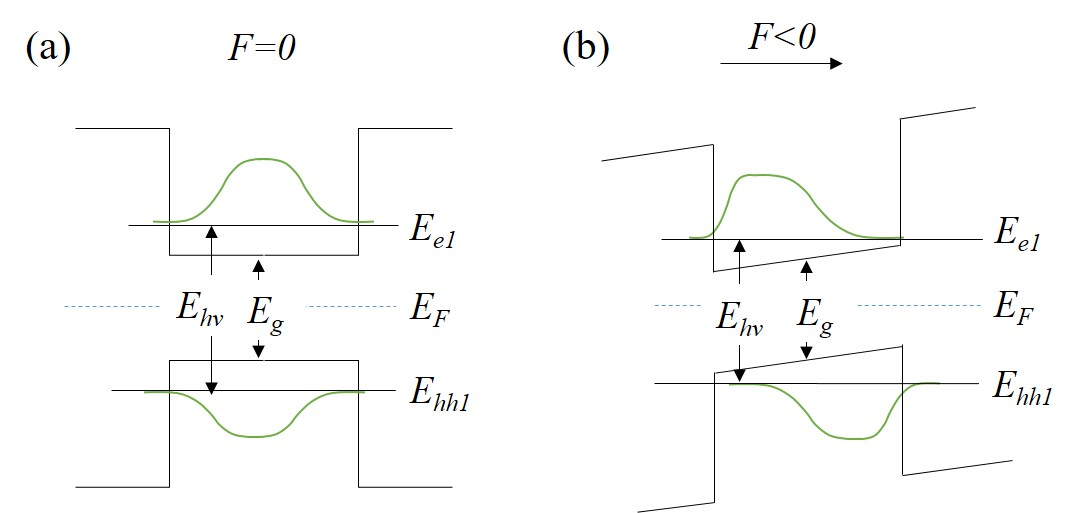
\includegraphics[width=14cm]{./Pictures/fig_ch2_band_lineup.jpg}
	\caption{ 量子阱的能带和波函数的示意图(a)有外界无电场下;(b)在外界电场的时候}
	\label{fig_ch2_band_lineup}
\end{figure}

图\ref{fig_ch2_band_lineup}(a)展示了没有外界偏压下量子阱的导带和价带,电子和空穴的波函数在空间上相互重叠,此时激子效应强度最大。当在外界电场的相互作用下,可以看到电子和空穴的分立能级的间隔变小,并且两者的波函数在空间上相错,此时激子效应的强度减弱。图\ref{fig_ch2_absorption_spec}(a,b)展示了实验测的不同偏振下量子阱的吸收谱随着外界电场的变化而变化\cite{chao1993momentum}。从中我们可以看出,外界电场使吸收谱往红移动,然后吸收谱边缘的激子吸收峰逐渐减弱,并且不同偏振下的吸收谱不同。图\ref{fig_ch2_absorption_spec}(c,d)展示了根据实验数据,里面计算得到的结果\cite{chao1993momentum}。可以看到理论和实验吻合的很好。关于量子阱中QCSE现象自从1984年在半导体量子阱材料被发现以来调\cite{miller1984band, wood1984high},依旧构建了多套完整的物理模型\cite{chuang1995physics}。下面,我们将介绍本论文采用的物理模型和计算方法。
\begin{figure}[htb]
	\centering
	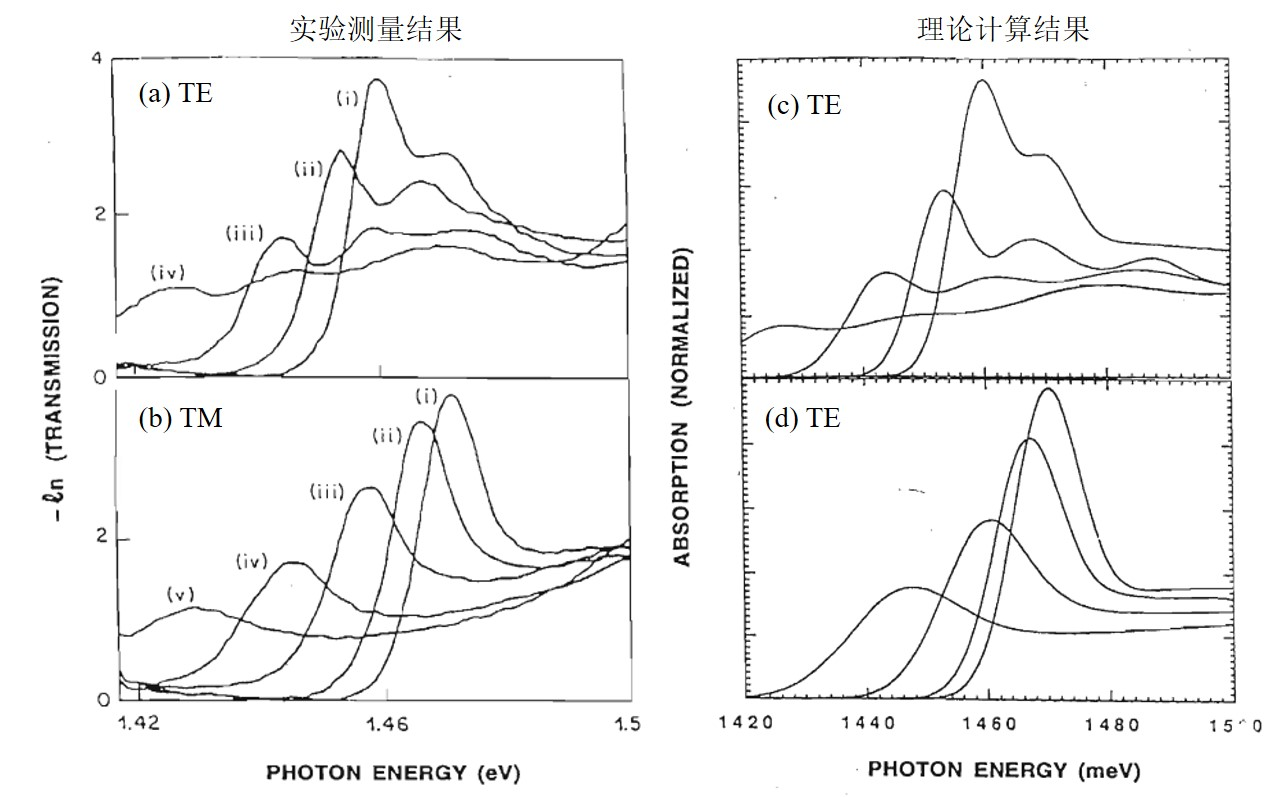
\includegraphics[width=14cm]{./Pictures/fig_ch2_absorption_spec.jpg}
	\caption{ (a,b) 实验测量的量子阱TE和TM偏振光的吸收谱\cite{chao1993momentum};(c,d) 理论计算的量子阱TE和TM偏振光的吸收谱\cite{chao1993momentum}}
	\label{fig_ch2_absorption_spec}
\end{figure}

\subsection{基本物理和数值计算}
目前计算量子阱的吸收谱商业上的软件只有一款昂贵的Harold EAM\cite{HarolEAM}软件。在此,我们采用文献[\citenum{chuang1995physics, mares1993modeling, roy1993modified, chuang1991exciton}]的方法,计算外界电场下的量子阱的吸收谱。计算吸收谱需要采用四个步骤,如图\ref{fig_ch2_flow_chart}(a)所示。通过第一步和第二布求解电子,空穴在外界下电场下的薛定谔方程\ref{Equ:Schro}得到本征能量$E$和波函数$\psi(z)$,如图\ref{fig_ch2_flow_chart}(b)所示。通过第三步和第四步求解出包含激子效应量子阱的吸收谱。
\begin{figure}[htb]
	\centering
	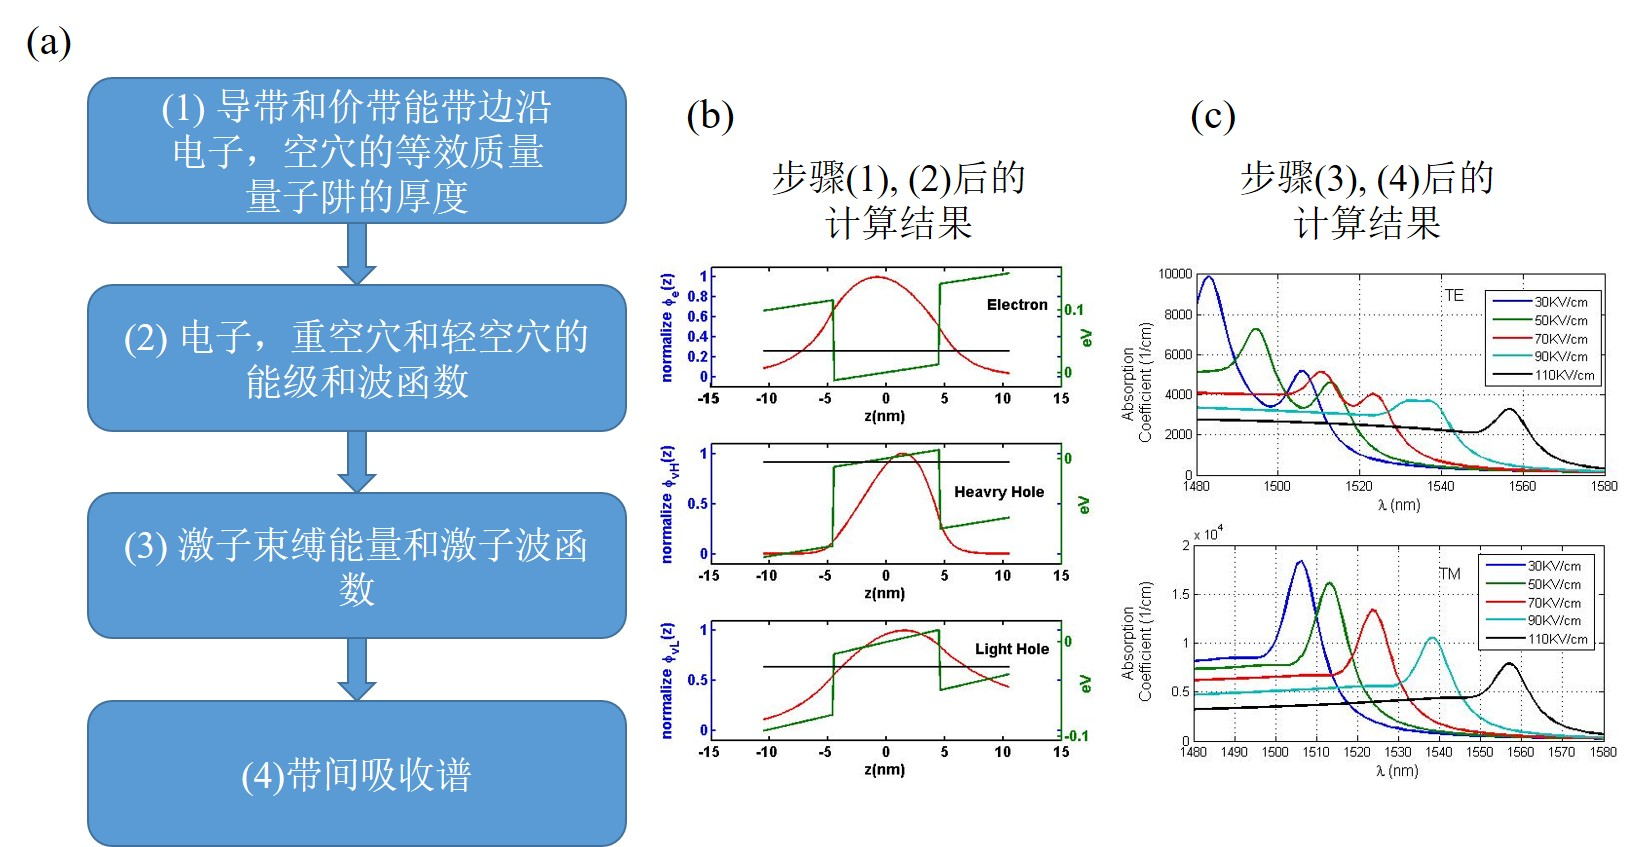
\includegraphics[width=16cm]{./Pictures/fig_ch2_flow_chart.jpg}
	\caption{(a)量子阱吸收谱的数值计算步骤;(b)第一和第二步的计算得到的电子,重空穴和轻空穴的能量和波函数;(c)第三和第四步计算得到的TE和TM偏振光的吸收谱}
	\label{fig_ch2_flow_chart}
\end{figure}

\begin{equation}
\label{Equ:Schro}
(\frac{\hbar^2}{2m}\Delta^2+V(z)+eFz)\psi(z)=E\psi(z)
\end{equation}
第一步计算材料的导带和价带的边沿结构。量子阱是由两种材料间隔排列而成。图\ref{fig_ch2_band_diagram}展示了在材料应力情况下量子阱能带边沿结构的变化\cite{chuang1995physics}。

\begin{figure}[htb]
	\centering
	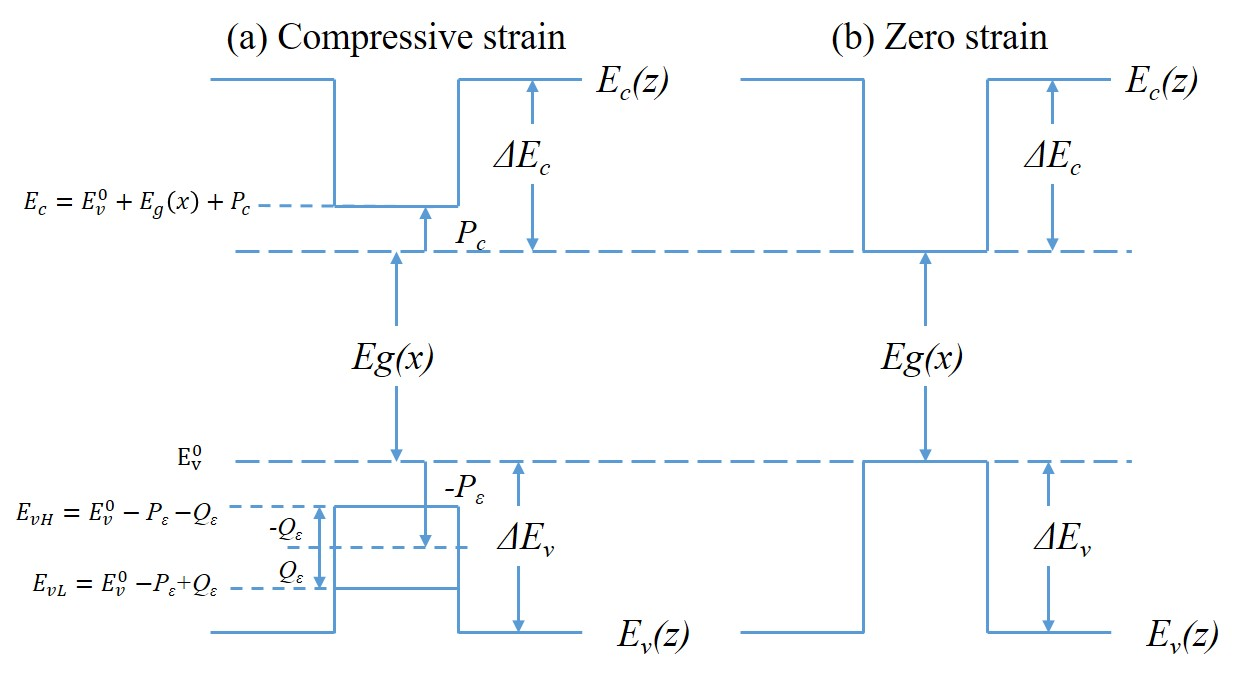
\includegraphics[width=14cm]{./Pictures/fig_ch2_band_diagram.jpg}
	\caption{有应力量子阱中的能带边沿图,(a)压缩应变;(b)张力应变}
	\label{fig_ch2_band_diagram}
\end{figure}

假设势阱中材料的晶格常熟为$a$,它在衬底晶格常数为$a_{0}$的材料上生长。那么我们可以用三个方向的应力来表式:
\begin{equation}
\label{Equ:exx}
\epsilon_{xx} = \epsilon_{yy} = \frac{a_{0}-a}{a}
\end{equation}
\begin{equation}
\label{Equ:ezz}
\epsilon_{zz} = -2\frac{C_{12}}{C_{11}}\epsilon_{xx}
\end{equation}
其中$C_{11}$和$C_{12}$是材料的弹性刚性常数(Elastic Stiffness Constants)。当$\epsilon_{zz}>0$时,材料处于压缩应变(Compressive Strain);当$\epsilon_{zz}>0$时,材料处于拉伸应变(Tensile Strain)。图\ref{fig_ch2_band_diagram}(a,b)展示了量子阱在有压缩应变和无应变情况下的能带的变化。通过比较,我们可以看到,导带上能带边沿$E_c$在受到压缩应变时,移动了$P_{c}$。表达式如下:
\begin{equation}
\label{Equ:Pc}
P_{c} = a_{c}(\epsilon_{xx}+\epsilon_{yy}+\epsilon_{zz})
\end{equation}
\begin{equation}
\label{Equ:Econ}
E_{c} = E_{v}^{0}(x)+E_{g}(x)+P_{c}
\end{equation}
其中$a_{c}$是导带的变形势能(Deformation Potentials),$E_v^0(x)$是材料在没有应变时导带的边沿,$E_{g}(x)$是材料没有应变时的导带和价带间隔,他们需要通过实验测试或者依旧材料的基本组分x查表拟合获得\cite{chuang1995physics,li2000material}。

在价带上,收到应变的影响,空穴分裂成重空穴和轻空穴,能带边沿分别是$E_{hh}$和$E_{lh}$。它们能带边沿的均值移动量是$P_{\epsilon}$,裂量是$Q_{\epsilon}$。具体表达式如下:
\begin{equation}
\label{Equ:Pe}
P_{\epsilon} = -a_{v}(\epsilon_{xx}+\epsilon_{yy}+\epsilon_{zz})
\end{equation}
\begin{equation}
\label{Equ:Qe}
Q_{\epsilon} = -\frac{b}{2}(\epsilon_{xx}+\epsilon_{yy}-2\epsilon_{zz})
\end{equation}
\begin{equation}
\label{Equ:Ehh}
E_{hh} = E_{v}^{0}(x)-P_{\epsilon}-Q_{\epsilon}
\end{equation}
\begin{equation}
\label{Equ:Elh}
E_{lh} = E_{v}^{0}(x)-P_{\epsilon}+Q_{\epsilon}
\end{equation}
其中$a_{v}$和$b$是变形势能。利用公式\ref{Equ:Econ},\ref{Equ:Ehh}、\ref{Equ:Elh}计算量子阱两种材料的能带边缘,就可以获得薛定谔方程中的电子,轻空穴和重空穴的势能$V(z)$。

在应力作用下,由于重空穴和轻空穴产的能带生劈裂,其等效质量,我们需要采用Luttinger parameters$\gamma_1, \gamma_2$计算。如下式所示:
\begin{equation}
\label{Equ:eff_mass_z}
\frac{m_{hh}^z}{m_0}=\frac{1}{\gamma_1-2\gamma_2}~~~~~~~~~~\frac{m_{lh}^z}{m_0}=\frac{1}{\gamma_1+2\gamma_2}
\end{equation}
\begin{equation}
\label{Equ:eff_mass_xy}
\frac{m_{hh}^{xy}}{m_0}=\frac{1}{\gamma_1+\gamma_2}~~~~~~~~~~\frac{m_{lh}^{xy}}{m_0}=\frac{1}{\gamma_1-\gamma_2}
\end{equation}
其中公式\ref{Equ:eff_mass_z}和公式\ref{Equ:eff_mass_xy}分别是计算垂直与量子阱方向(即z方向)和水平方向重空穴和轻空穴的等效质量\cite{eppenga1987new}。

我们用于硅基混合集成III-V电吸收光调制器的多量子阱中,单个量子阱的势阱(Well)和势垒(Barrier)分别是:In\SB{0.65}Al\SB{0.09}Ga\SB{0.26}As和In\SB{0.42}Al\SB{0.17}Ga\SB{0.39}As。从文献[\citenum{chuang1995physics,li2000material}],根据它们各个元素,再依据\ref{Equ:Econ},\ref{Equ:Ehh}、\ref{Equ:Elh}、\ref{Equ:eff_mass_z}、\ref{Equ:eff_mass_xy}式可以获得如下表\ref{QWmaterial}的量子阱材料数据。其中势阱受到了0.82\%的压缩应变,势垒受到了0.73\%的拉伸应变。
{
	\begin{table}[htb]
		\zihao{5}
		\caption{量子阱材料数据。E\SB{lh}:轻空穴的能带边沿;E\SB{hh}:重空穴的能带边沿;E\SB{c}:导带的能带边沿;$m_{lh}^z$:轻空穴z向等效质量;$m_{lh}^{xy}$:轻空穴xy向等效质量;$m_{hh}^z$:重空穴z向等效质量;$m_{hh}^{xy}$:重空穴xy向等效质量;$m_e$:电子等效质量;$m_0$:电子质量。}
		\label{QWmaterial}
		\centering
		\begin{tabular}[t]{ccccccccc}
			\hline
			类型  & E\SB{lh}(eV) & E\SB{hh}(eV) & E\SB{c}(eV) & $m_{lh}^z$ ($m_0$) & $m_{lh}^{xy}$ ($m_0$) & $m_{hh}^{z}$ ($m_0$) & $m_{hh}^{xy} $ ($m_0$) & $m_e$ ($m_0$)\\
			\hline
			Well & -6.7220 & -6.6695 & -5.9031 & 0.0374 & 0.1216 & 0.4874 & 0.0486 & 0.0457\\
			Barrier& -6.7573 & -6.8114 & -5.7680 & 0.0481 & 0.1498 & 0.5080 & 0.0621 & 0.0641\\
			\hline
		\end{tabular}
	\end{table}
}

第二步数值求解公式\ref{Equ:Schro}计算电子,重空穴和轻空穴在在一维势阱中的能级和波函数。在此我们采用的是基于传输矩阵的求解方法\cite{chuang1995physics}。首先我们将势能$V(z)+eFz$均匀分解很小的区域如图\ref{fig_ch2_divide_potential}所示。
\begin{figure}[htb]
	\centering
	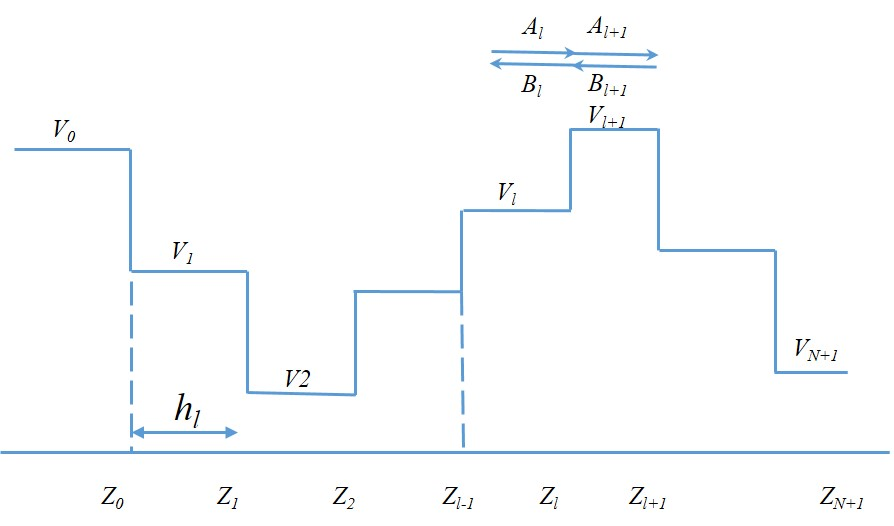
\includegraphics[width=12cm]{./Pictures/fig_ch2_divide_potential.jpg}
	\caption{将势能均匀划分成很小区域的示意图}
	\label{fig_ch2_divide_potential}
\end{figure}

假设在区域$l$,$z_{l-1} \leqslant z \leqslant z_{l}$,势能为$V_l$,粒子质量为$m_l$,那么其波函数$\psi(z)$的通解为:
\begin{equation}
\label{Equ:generalsolutionsch}
\psi(z) = A_le^{ik_l(z-z_l)}+B_le^{-ik_l(z-zl)}
\end{equation}
其中区域$l$的波数$k_l$可以用本征能量$E$来表示:
\begin{equation}
\label{Equ:kl}
k_l = \sqrt{\frac{2m_l}{\hbar^2}(E-V_l)}
\end{equation}
再利用每个区域边间上$\psi(z)$和$(1/m(z))d\psi(z)/dz$连续的条件,我们可以获得区域$l+1$的系数$A_{l+1}$和$B_{l+1}$与区域$l$的系数$A_l$和$B_l$的关系:
\begin{equation}
\label{Equ:ABrelation}
\begin{bmatrix}
A_{l+1}\\
B_{l+1}
\end{bmatrix} = \textbf{F}_{(l+1)l}\begin{bmatrix}
A_{l}\\
B_{l}
\end{bmatrix}
\end{equation}
其中$\textbf{F}_{(l+1)l}$可以表示为:
\begin{equation}
\label{Equ:Fdetail}
\textbf{F}_{(l+1)l} = \frac{1}{2}\begin{bmatrix}
(1+P_{(l+1)l})e^{ik_{l+1}h_l}&(1-P_{(l+1)l})e^{ik_{l+1}h_l}\\
(1-P_{(l+1)l})e^{-ik_{l+1}h_l}&(1+P_{(l+1)l})e^{-ik_{l+1}h_l}
\end{bmatrix}
\end{equation}
其中$P_{(l+1)l}$可以表示为:
\begin{equation}
\label{Equ:Pdetail}
P_{(l+1)l} = \frac{m_lk_{l+1}}{m_{l+1}k_{l}}
\end{equation}
因此,我们可以得到第一个区域系数$A_{0}$和$B_{0}$和最后一个区域系数$A_{N+1}$和$B_{N+1}$的关系:
\begin{equation}
\label{Equ:Fmulti}
\begin{bmatrix}
A_{N+1}\\
B_{N+1}
\end{bmatrix} = \textbf{F}_{(N+1)N}\textbf{F}_{N(N-1)}\cdots\textbf{F}_{21}\textbf{F}_{10}\begin{bmatrix}
A_{0}\\
B_{0}
\end{bmatrix}
\end{equation}
由于第一区域和最后区域波函数一般要衰减的,因此$A_0 = 0$,$B_{N+1} = 0$。另外我们将矩阵的连乘写成如下形式:
\begin{equation}
\label{Equ:Fsimple}
\textbf{F}_{(N+1)N}\textbf{F}_{N(N-1)}\cdots\textbf{F}_{21}\textbf{F}_{10} = \begin{bmatrix}
f_{11}&f_{12}\\
f_{21}&f_{22}
\end{bmatrix}
\end{equation}
因此公式\ref{Equ:Fmulti}可以写成如下形式:
\begin{equation}
\label{Equ:Fmulti}
\begin{bmatrix}
A_{N+1}\\
0
\end{bmatrix} = \begin{bmatrix}
f_{11}&f_{12}\\
f_{21}&f_{22}
\end{bmatrix}
\begin{bmatrix}
0\\
B_{0}
\end{bmatrix}
\end{equation}
因此,我们获得了求解借本征量能$E$的方程:
\begin{equation}
\label{Equ:sloveE}
f_{22}(E) = 0
\end{equation}
利用牛顿迭代法或者其他数值方法我们可以获得$E$的数值。然后公式\ref{Equ:kl},\ref{Equ:Pdetail},\ref{Equ:Fdetail}反推得到$\textbf{F}$。再假设$B_{0}$的数值,利用公式\ref{Equ:Fmulti},我们就可以得到每个区域波函数$\psi(z)$。最后,根据粒子在整个空间出现的概率为1,对波函数进行归一化。图\ref{fig_ch2_bias_wavefunction}分别展示了在没有偏压和2 KV/cm的偏压下,利用传输矩阵,计算得到的电子,重空穴,轻空穴的最低能级和对应波函数,其中量子阱势阱的宽度 $t_w = 11 ~nm$。在没有偏压下,电子和重空穴之间的能量间隔是$E_{e-hh} = 0.7997 ~eV$,当偏压为18~ KV/cm时,其间隔变为$E_{e-hh} = 0.7982~eV$,表明吸收峰红移了$\Delta E_{e-hh} = 1.5 ~meV$。电子和轻空穴在没有偏压和18 ~KV/cm下的能量间隔$E_{e-lh}$分别是$0.8649 eV$和$0.8597 eV$,红移量为 $\Delta E_{e-lh} = 5.2~ mV$。$\Delta E_{e-lh}$ 大于 $\Delta E_{e-hh}$是由于,如表\ref{QWmaterial}所示,轻空穴的等效质量少于重空穴,并且轻空穴的势垒和势阱的能带变差相比重空穴而言更小,因此轻空穴更容易受到势能变化的影响。从图\ref{fig_ch2_bias_18KV_wf}的最后一幅轻空穴的波函数图中可以看出,轻空穴即将突破量子阱势垒的束缚。当外界电场很强时,由于粒子会有部分从势阱里逃逸,此时波函数无法用公式\ref{Equ:generalsolutionsch}来表示,需要采用Airy方程表示此时波函数的通解\cite{chuang1991exciton}。
%\begin{figure}[htb]
%	\centering
%	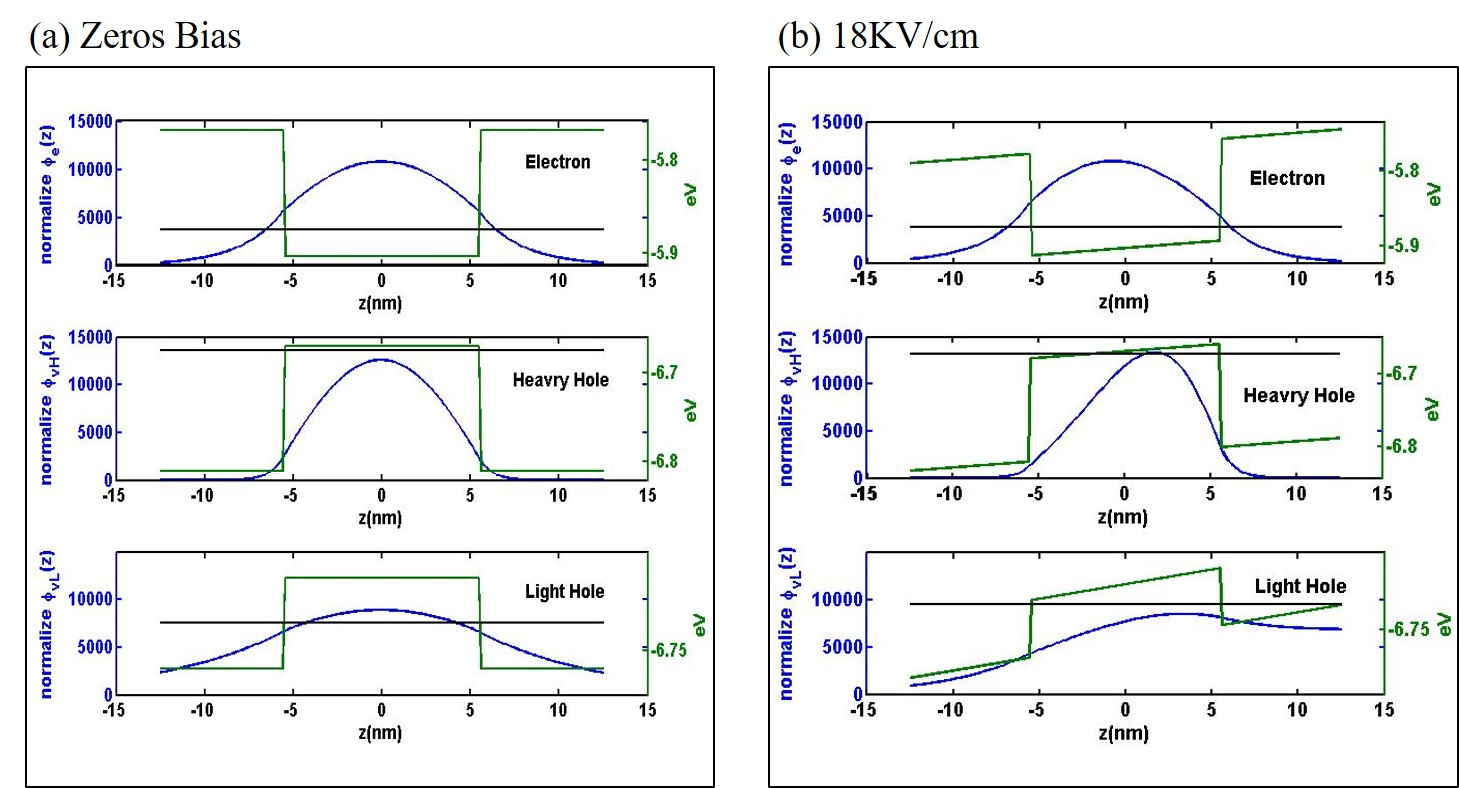
\includegraphics[width=16cm]{./Pictures/fig_ch2_bias_wavefunction.jpg}
%	\caption{在不同偏压下电子,重空穴和轻空穴能带边沿,波函数,能级的变化,(a)无电场;(b)电场强度为18~ KV/cm}
%	\label{fig_ch2_bias_wavefunction}
%\end{figure}

\begin{figure}[htb]
	\small
	\subfigure[0~KV/cm]{
		\begin{minipage}[]{0.5\textwidth}
			\centering
			\label{fig_ch2_bias_0KV_wf}
			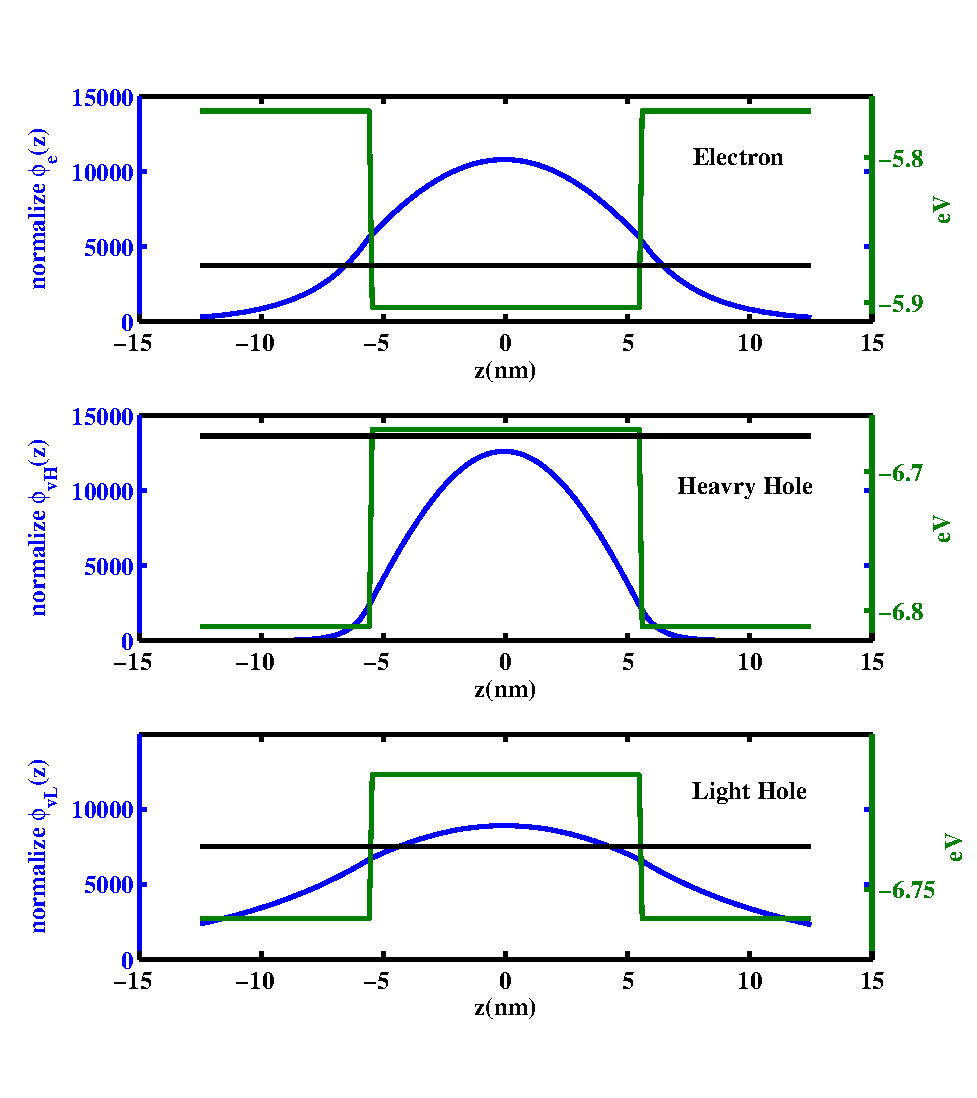
\includegraphics[width=8cm]{./Pictures/fig_ch2_bias_0KV_wf.eps}
		\end{minipage}}
	\subfigure[18~KV/cm]{
		\begin{minipage}[]{0.5\textwidth}
			\centering
			\label{fig_ch2_bias_18KV_wf} %% label for second subfigure
			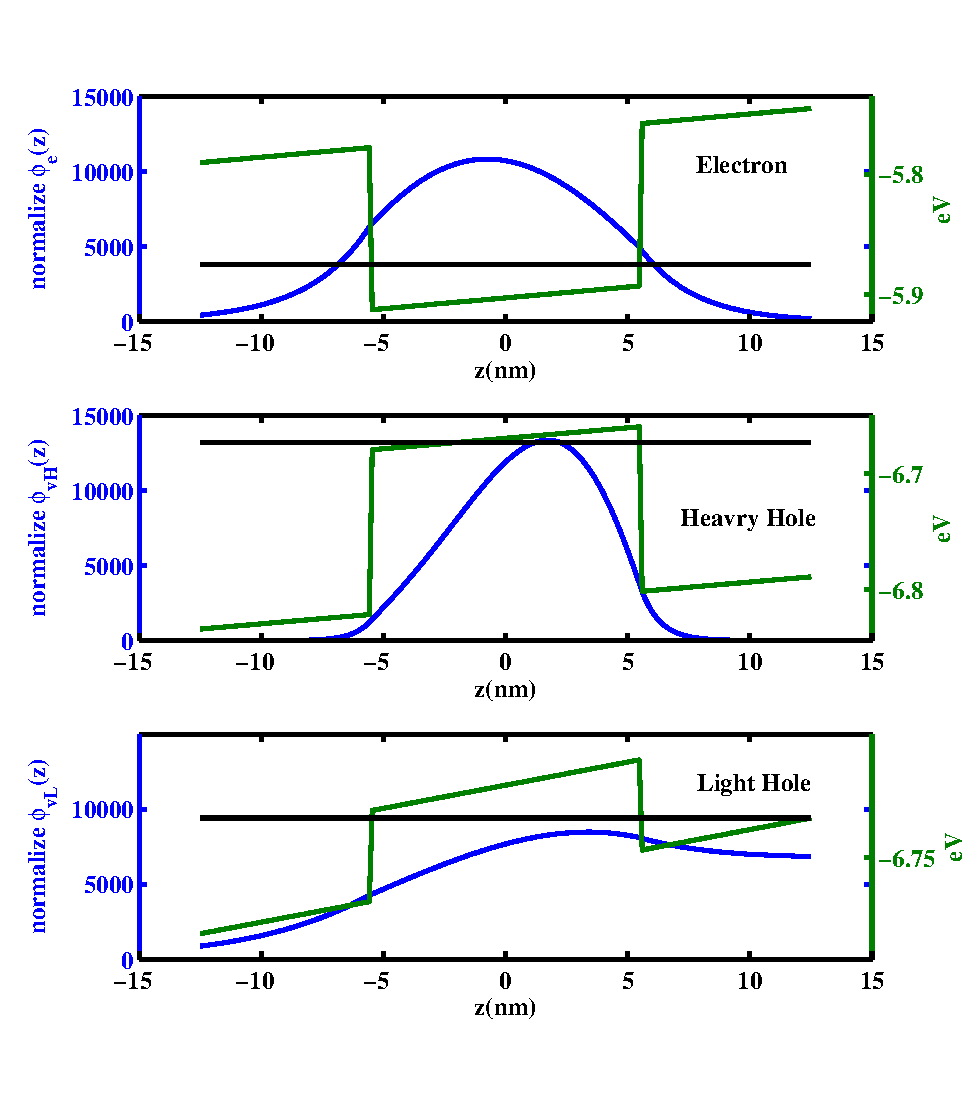
\includegraphics[width=8cm]{./Pictures/fig_ch2_bias_18KV_wf.eps}
		\end{minipage}}
	\caption{在不同偏压下电子,重空穴和轻空穴能带边沿,波函数,能级的变化}
	\label{fig_ch2_bias_wavefunction}	
\end{figure}
		
第三步求解激子的束缚能$E_B$和激子波函数$\psi(\rho)$。$\rho$是电子和空穴的xy平面上的距离。量子阱吸收谱的边缘处的能量$E_{e-h}$由能带间隔$E_g$,电子的能级$E_e$,空穴的能级$E_h$,激子束缚能$E_B$确定的,如下式所示:
\begin{equation}
\label{Equ:Eeh}
E_{e-h} = E_g + E_e + E_h + E_B
\end{equation}

求解$E_B$和$\psi(\rho)$需要解含电子空穴在库仑动能中的薛定谔方程\cite{mares1993modeling}。可以通过变法发求解这个方程\cite{miller1985electric, mares1993modeling}。最后可以转化为求解公式\ref{Equ:EB_lambda}的最小值问题。
\begin{equation}
\label{Equ:EB_lambda}
E_B(\lambda)=\frac{\hbar^2}{2\mu\lambda^2}-\frac{e^2}{4\pi\epsilon_r\epsilon_0}\int_{ - \infty }^{ \infty } {dz_e}\int_{ - \infty }^{ \infty } {dz_h	\left| \psi_e(z_e) \right|^2\left| \psi_h(z_h) \right|^2}\int_{ 0 }^{ \infty }{dq\frac{e^{-q\left| z_e-z_h \right|}}{\left[1+\left( \lambda q/2 \right) ^2 \right]^{3/2}}}
\end{equation}
其中$\lambda$是变分法中的变分参数。激子波函数$\psi(\rho)$可以用变分参数$\lambda$表示为:
\begin{equation}
\label{Equ:psirho}
\psi(\rho)=\sqrt{2/\pi}\left(e^{-\rho/\lambda}/\lambda \right)
\end{equation}

图\ref{fig_ch2_ex_abs1}和图\ref{fig_ch2_ex_abs2}展示了,在有激子和没有激子效应下,量子阱中$E_{e-hh}$与$E_{e-lh}$所对应的吸收峰边沿随外界电场的漂移。可以看出不考虑激子效应的吸收峰边沿比实际的吸收峰往短波偏,但是两者的吸收峰边沿在外界电压的变化下,都以二次函数的关系进行红移。可以总结出,激子的束缚能随外界电场的变化量远小于电子和空穴能级间隔的变化量。
\begin{figure}[htb]
	\centering
	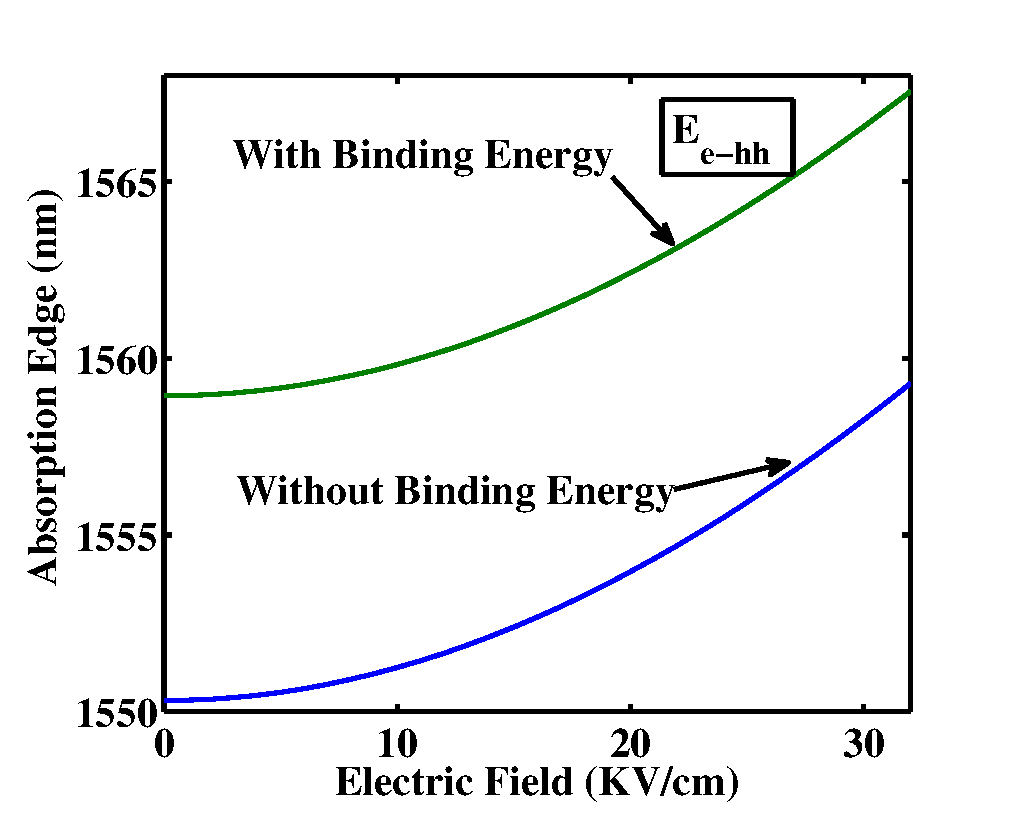
\includegraphics[width=12cm]{./Pictures/fig_ch2_ex_abs1.eps}
	\caption{$E_{e-hh}$所对应吸收峰边沿没有和存在激子效应下,随外界电场的变化}
	\label{fig_ch2_ex_abs1}
\end{figure}
\begin{figure}[htb]
	\centering
	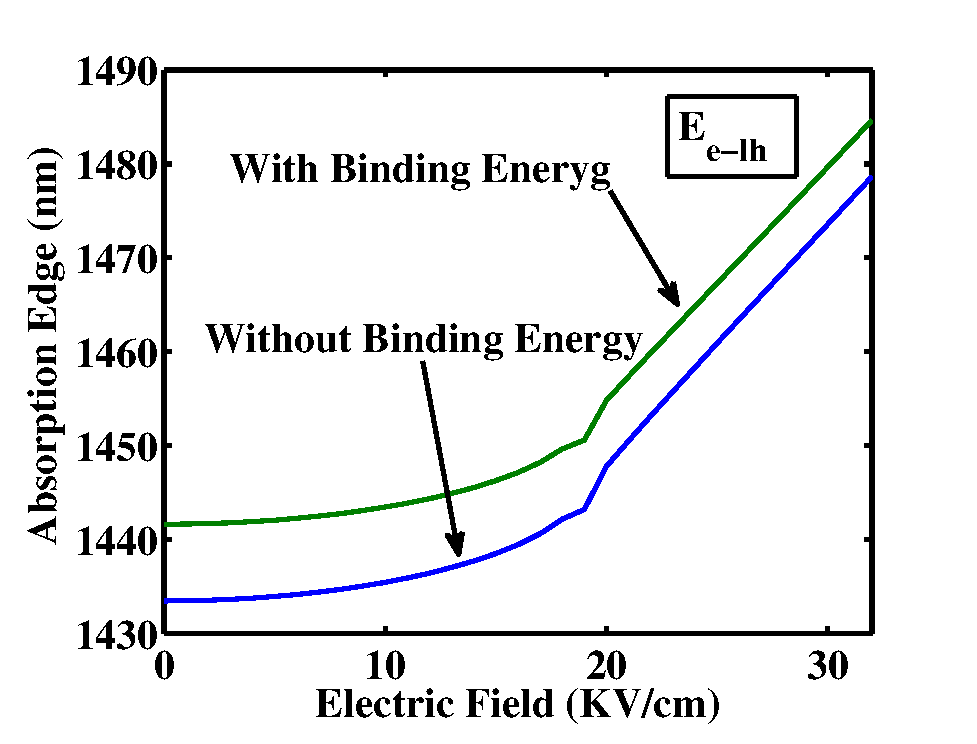
\includegraphics[width=12cm]{./Pictures/fig_ch2_ex_abs2.eps}
	\caption{$E_{e-lh}$所对应吸收峰边沿没有和存在激子效应下,随外界电场的变化}
	\label{fig_ch2_ex_abs2}
\end{figure}

第四步求解量子阱带间跃迁的吸收谱。带间电子能级$n$和空穴能级$m$的跃迁吸收谱可以简化成两个部分,第一个部分是带间连续跃迁导致的连续吸收谱,如公式\ref{Equ:continuumabs}所示;第二个部分是激子跃迁产生的激子吸收谱,如公式\ref{Equ:excitonabs}所示。
\begin{equation}
\label{Equ:continuumabs}
\begin{aligned}
\alpha(\omega) = &\frac{\omega \mu e^2}{n_rc\epsilon_0\pi m_0^2 L_p} \sum_m\sum_n\left| I_{nm} \right|^2\left| M_{AVG} \right|^2 \\ & \int_{0}^{\infty}\frac{dE~M(E)S_{nm}\Gamma}{(E_g+E_m+E_n+E)^2[(E_g+E_m+E_n+E-\hbar\omega)^2+\Gamma^2]}
\end{aligned}
\end{equation}

\begin{equation}
\label{Equ:excitonabs}
\alpha(\omega) = \frac{2\omega e^2 \hbar^2}{n_r c \epsilon_0 m_0^2 L_p} \sum_{mn}\frac{M(E)|M_{AVG}|^2|I_{nm}|^2|\psi(\rho = 0)^2|^2\Gamma}{(E_g+E_m+E_n+E_B)^2[(E_g+E_m+E_n+E_B-\hbar\omega)^2+\Gamma^2]}
\end{equation}
其中,$I_{nm}$是电子和空穴对应能级的波函数的重叠积分
\begin{equation}
\label{Equ:Imn}
I_{nm} = \left< \psi_n(z)|\psi_m(z)\right>,
\end{equation}
$|M_{AVG}| ^2$是布洛赫模式的平均矩阵量
\begin{equation}
\label{Equ:MAVG}
\left| M_{AVG} \right| ^2 = \frac{m_0}{6} \left( \frac{m_0}{m^*}-1\right)\frac{E_g(E_g+\Delta)}{E_g+(2\Delta/3)},
\end{equation}
其中,$\Delta$是自旋轨道分裂能(spin-orbit split-off energy),$L_p$是量子阱的单个周期长度,$m_0$是电子的静止能量,$\mu = (1/m_e+1/m_{h}^xy)$是约化有效质量, $S_{nm}$是库仑增强因子,$M(E)$具有偏振相关性\cite{chuang1991exciton, yamanishi1984comment, asada1984gain}。对于TE偏振的$M(E)$见表\ref{METE}:
{
	\begin{table}[htb]
		\zihao{5}
		\caption{TE偏振的$M(E)$}
		\label{METE}
		\centering
		\begin{tabular}[t]{p{3cm}cc}
			\hline
			     & 重空穴 & 轻空穴 \\
			\hline
			连续跃迁  & $\frac{3}{4} \left[ 1+ \left( \frac{E_m + E_n}{E_m+E_n+E}\right)\right]$ & $\frac{1}{4} \left[ 5-3 \left( \frac{E_m + E_n}{E_m+E_n+E}\right)\right]$ \\
			激子跃迁  & $\frac{3}{2}$ & $\frac{1}{2}$\\
			\hline
		\end{tabular}
	\end{table}
}

对于TM偏振的$M(E)$见表\ref{METM}:
{
	\begin{table}[htb]
		\zihao{5}
		\caption{TM偏振的$M(E)$}
		\label{METM}
		\centering
		\begin{tabular}[t]{p{3cm}cc}
			\hline
			& 重空穴 & 轻空穴 \\
			\hline
			连续跃迁  & $\frac{3}{2} \left[ 1- \left( \frac{E_m + E_n}{E_m+E_n+E}\right)\right]$ & $\frac{1}{2} \left[ 1+3 \left( \frac{E_m + E_n}{E_m+E_n+E}\right)\right]$ \\
			激子跃迁  & 0 & 2\\
			\hline
		\end{tabular}
	\end{table}
}

结合公式\ref{Equ:continuumabs}和公式\ref{Equ:excitonabs}我们可以获得量子阱在电场下的总吸收谱。我们仿真量子阱(In\SB{0.65}Al\SB{0.09}Ga\SB{0.26}As和In\SB{0.42}Al\SB{0.17}Ga\SB{0.39}As分别作为势阱和势垒)的TE模式的吸收谱见图\ref{fig_ch2_te_abs},TM模式的吸收谱见图\ref{fig_ch2_tm_abs}。作为电吸收光调制器,我们最关注的是吸收谱边沿的变化,因此仿真吸收谱时,我们只考虑了电子,重空穴和轻空穴最低的能级和对应的波函数。吸收谱的宽度因子$\Gamma$根据实验数据拟合,其随外界电场的变化而展宽;外界电场为0时,$ \Gamma = 1 ~meV$;外界电场为32 KV时,$ \Gamma = 1.3 ~meV$。库仑增强因子是1~2的范围内\cite{mares1993modeling, chuang1995physics},在此我们取2。公式\ref{Equ:MAVG}中的等效质量$m^* = 0.14m_{e—well}$ ($m_{e-well}$是势阱中的等效电子质量)。

\begin{figure}[htb]
	\centering
	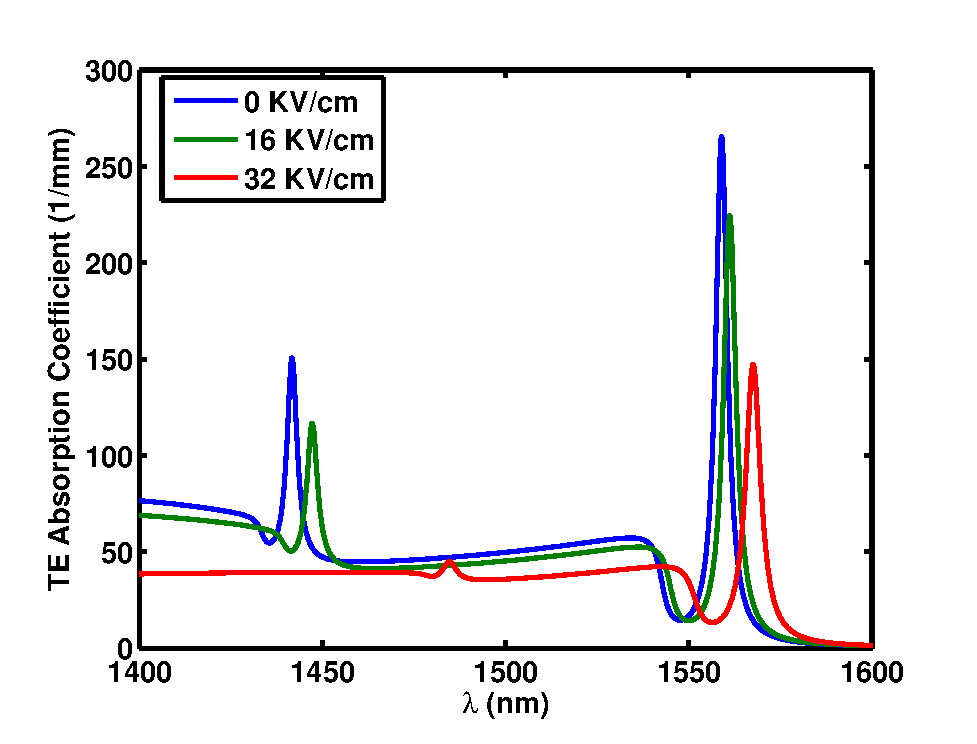
\includegraphics[width=12cm]{./Pictures/fig_ch2_te_abs.eps}
	\caption{TE模式的吸收谱}
	\label{fig_ch2_te_abs}
\end{figure}
\begin{figure}[htb]
	\centering
	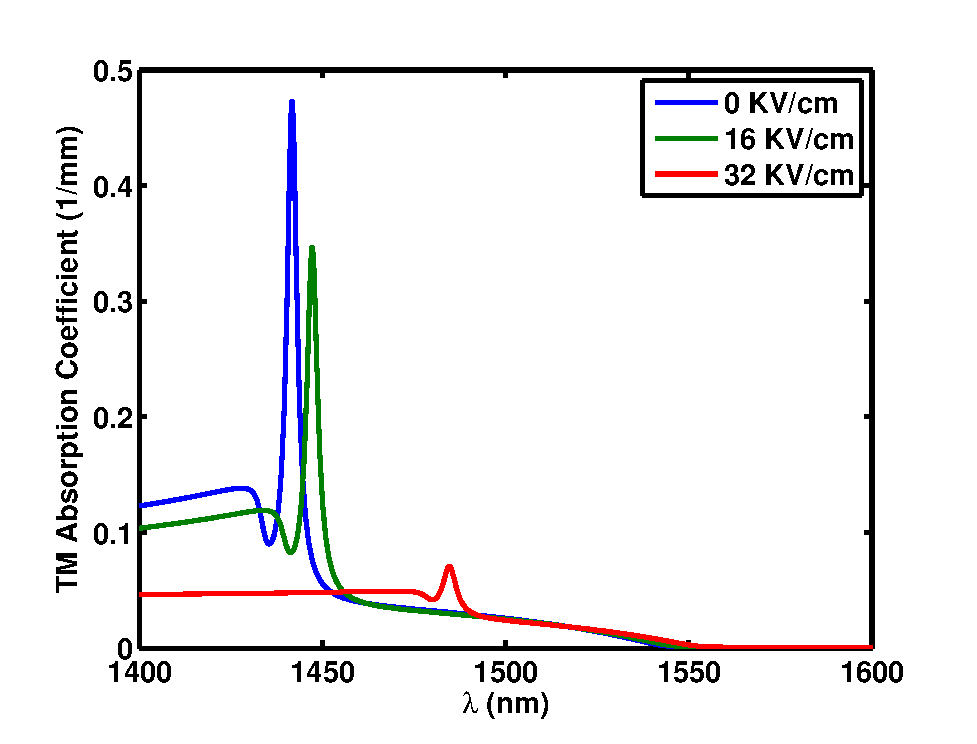
\includegraphics[width=12cm]{./Pictures/fig_ch2_tm_abs.eps}
	\caption{TM模式的吸收谱}
	\label{fig_ch2_tm_abs}
\end{figure}

从图\ref{fig_ch2_te_abs}我们可以看出,量子阱TE偏振吸收谱边沿有强烈的激子吸收峰,并且随着电场的增强往长波移动,其对应的是电子和重空穴跃迁的能量$E_{e-hh}$如图\ref{fig_ch2_ex_abs}(a)所示。而1.45 $\mu m$处对应的小吸收峰是电子和轻空穴跃迁的能量$E_{e-lh}$如图\ref{fig_ch2_ex_abs}(b)。除此之外,激子吸收峰的强度在电场的作用下从$265 mm^{-1}$减弱到$147 mm^{-1}$。从图\ref{fig_ch2_tm_abs}我们可以看出,量子阱TM偏振吸收谱对应的是$E_{e-lh}$,激子吸收峰的强度从$473~ mm^{-1}$减弱到$70~ mm^{-1}$,这是由于轻空穴在强外界电场下从势阱中逃逸,导致轻空穴和电子波函数的叠加积分迅速降低,激子效应减弱。因此,在外界强电场下,高的势垒能,大的空穴与电子等效质量,能保持激子吸收峰的强度,但同时减弱了激子吸收峰随电场的偏移量。这也说明了电吸收调制器中,基于QCSE效应下,在相同长度的材料中,不采用谐振结构时,同时实现高消光比和低驱动电压的光调制器的矛盾。

\subsection{基于退火算法的优化设计}
在设计量子阱时,我们关注的是吸收谱边沿的位置,而设计量子阱的吸收谱边沿是一个多参数优化的问题,吸收谱的位置和量子阱中势阱的宽度$t_w$,以及材料的组分有关。比如我们采用的量子阱是In\SB{x}Al\SB{y}Ga\SB{1-x-y}As材料,势阱和势垒都需要2个参数确定。因此,设计量子阱的吸收谱边沿需要5个参数。在此我们采用了退火算法(Simulated annealing, SA)\cite{Kirkpatrick671}设计量子阱结构。退火算法可用于在受约束条件下寻找多参数的全局最优解。在使用退火算法时,需要注意约束条件的设计和权值函数的设计。合理的约束条件和权值函数能加快退火算法的收敛。

在此利用退火算法,设计了对TE和TM偏振有相同吸收边沿波长位于1530~ nm的量子阱,用于实现偏振不敏感的光调制。本文采用对材料的约束条件是势阱和势垒材料的约束条件相同:0.35 < x < 0.99,0.01 < y < 0.99。量子阱中势阱宽度的约束条件:8 nm < $t_w$ < 15 nm。我们的权值$f_{val}$的表达式如公式\ref{Equ:SAfunvalue}所示。
\begin{equation}
\label{Equ:SAfunvalue}
f_{val} = C_{TE}(\lambda_{TE}-\lambda_{0})^2 + C_{TM}(\lambda_{TM}-\lambda_{0})^2 + C_{diff}(\lambda_{TE}-\lambda_{TM})^2 + C_{w}(t_w-t_{w0})^2,
\end{equation}
其中$C_{TE}, C_{TM}$ 为计算得到的吸收峰边沿$\lambda_{TE}, \lambda_{TM}$与设计值$\lambda_{0}$偏差的权值函数; $C_{diff}$为TE和TM偏振吸收峰之间的距离的权值函数;$C_{w}$为优化得到的量子阱势阱宽度$t_w$和设计值之间的偏差的权值函数;在此我们取:$C_{TE} = C_{TM} = 20; C_{diff} = 100; C_{w} = 10$。由于退火算法是包含随机性,因此每次优化的时间都有所不同。图\ref{fig_ch2_fast_annealing}展示了退火算法的优化过程,可以看到经过了200次迭代,权值函数就已经达到稳定值236。
\begin{figure}[htb]
	\centering
	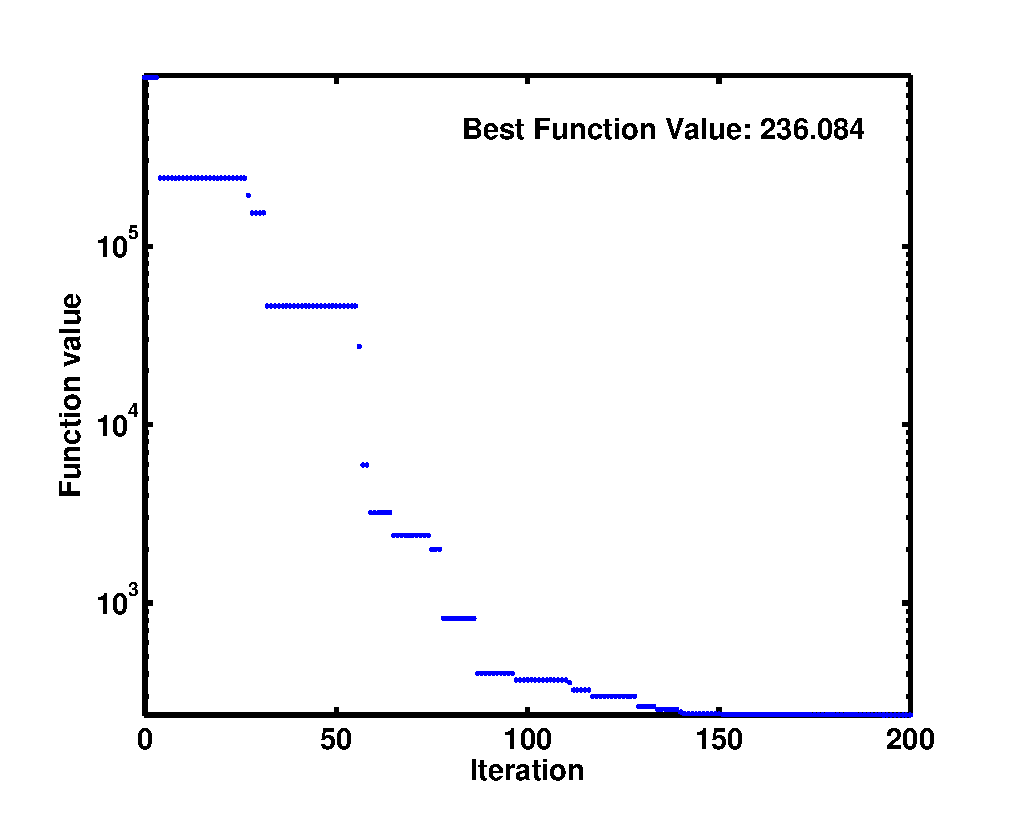
\includegraphics[width=12cm]{./Pictures/fig_ch2_fast_annealing.eps}
	\caption{退火算法的权值函数的优化过程}
	\label{fig_ch2_fast_annealing}
\end{figure}
此时对应量子阱的参数是:势阱$x = 0.495$, $y  = 0.01$;势垒$x = 0.521$,$y = 0.077$;量子阱势阱宽度$t_w = 9.5 nm$。其对应两个偏振吸收峰边沿的波长分别是$ \lambda_{TE} =1529.99~ nm, \lambda_{TM} =  1529.96 ~nm$,两者差值只有0.03nm。在考虑激子效应后,两者波长的分别是$ \lambda_{TE-ex} =1537.58~ nm, \lambda_{TM-ex} =  1538.49~ nm$,两者相差也只有0.91~nm。沿用之前计算吸收谱的参数,此量子阱的吸收谱如图\ref{fig_ch2_opt_abs_tetm},可以看到两个吸收峰位置几乎完全重合,而吸收谱强度的高低主要是由于轻空穴和重空穴波函数的不同,以及$M(E)$见表\ref{METE}和\ref{METM}。
\begin{figure}[htb]
	\centering
	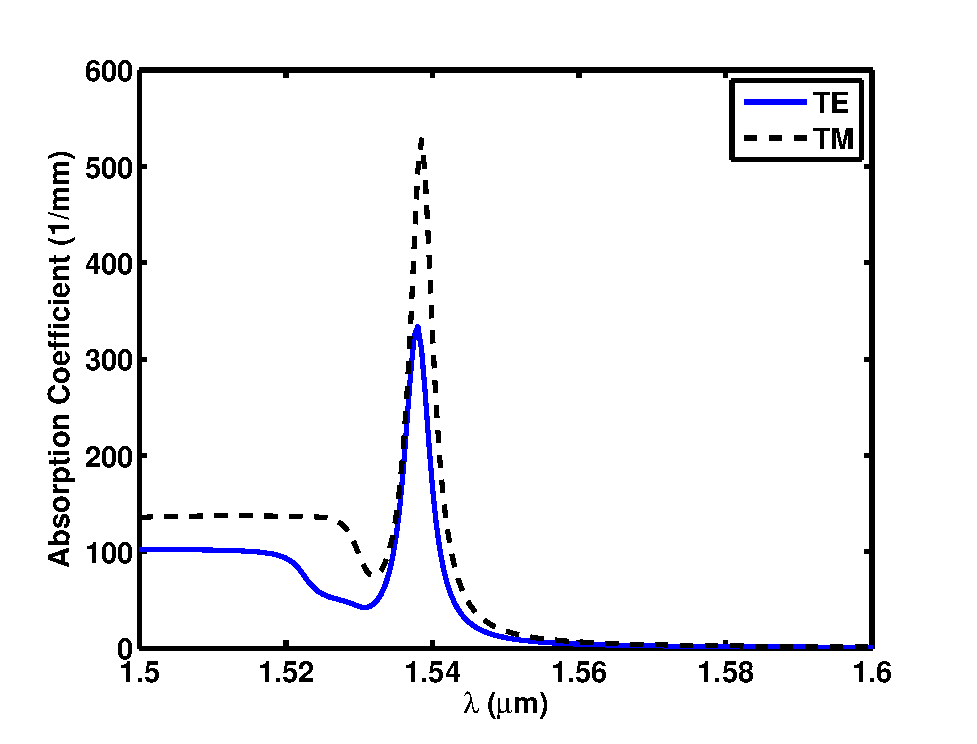
\includegraphics[width=12cm]{./Pictures/fig_ch2_opt_abs_tetm.eps}
	\caption{最后优化的量子阱对TE和TM偏振的吸收谱}
	\label{fig_ch2_opt_abs_tetm}
\end{figure}

\section{III-V外延片的总体设计}
III-V外延结构,不仅包含量子阱的设计,也也包p型重掺杂的欧姆接触层(p contact), 覆盖层(p cladding),隔离限制异质层(Separate Confinement Heterostructure, SCH),n参杂的欧姆接触层(n contact),如图\ref{fig_ch2_banddiagram}(a)所示。其中p contact层为InGaAs,用于和金属电极之间形成欧姆接触,掺杂浓度一般达到1.5$\times$10\SP{19} ~cm\SP{-3}。p cladding层为InP,SCH层是和量子阱相同元素的材料,但是它的折射率比量子阱偏小,能带间隔也偏大以防吸收多量子阱区域的光。SCH层也需要和InP衬底晶格匹配,避免产生额外的应力。p cladding和SCH共同作用使光场约束在多量子阱区域,防止光被重掺杂的p-cladding层和金属电极吸收。通常p pcladding层的厚度达到1.5~$\mu m$。
\begin{figure}[htb]
	\centering
	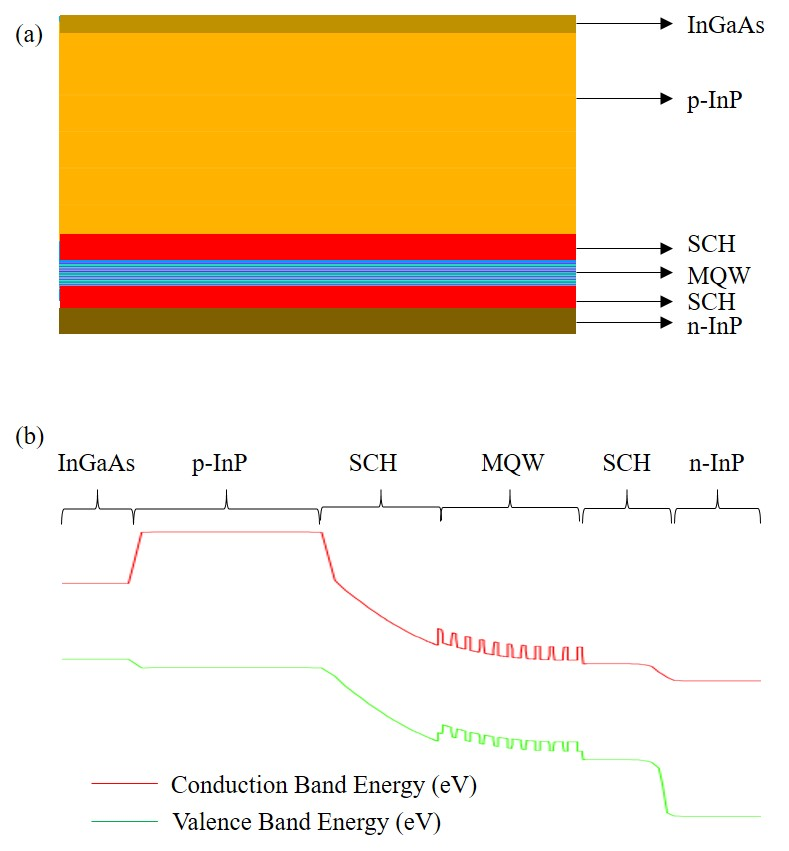
\includegraphics[width=12cm]{./Pictures/fig_ch2_banddiagram.jpg}
	\caption{(a)多量子阱外延片的结构示意图;(b)多量子阱外延片的能带示意图}
	\label{fig_ch2_banddiagram}
\end{figure}

图\ref{fig_ch2_banddiagram}(b)展示了多量子阱的能带示意图,其中量子阱区域能带的弯曲是由于内部p-i-n结的内建电场导致的。多量子阱是由多个量子阱叠加而成的,除了要设计单个单个量子阱的吸收峰外,我们还需要考虑实际工艺中多量子阱中的应力问题。虽然单个量子阱中势阱的应力无法避免,但是通过合理设计势垒的应力以及它的宽度,使总应力$S_{total}$变为0,能增强材料的可靠性\cite{chen2011high}。
\begin{equation}
\label{Equ:strain_net}
S_{total} = t_{w}\epsilon_{w}+t_b\epsilon_b
\end{equation}
其中,$t_{w}$和$t_{b}$分别是多量子阱中势阱和势垒的总厚度,$\epsilon_w$和$\epsilon_b$分别是势阱和势垒的应力。

\section{波导的设计}
在设计用于光调制器的硅基混合集成III-V波导时,我们不仅需要考虑波导在光学上的性能,比如传输损耗,约束因子,等效折射率,群折射率,还需要考虑微波信号传输的特性,比如特征阻抗,微波的等效折射率,传输线的等效电容和电阻。下面将分析矩形波导和蘑菇型波导的两种结构在光学和微波上的性能。这两种波导采用同样的材料参数如表所示\ref{epi_structure}\cite{yongbophd}:
{
	\begin{table}[htb]
		\zihao{5}
		\caption{III-V 波导的材料参数}
		\label{epi_structure}
		\centering
		\begin{tabular}[t]{lllll}
			\hline
			名称 & 厚度 ($\mu m$) & 折射率 n& \tabincell{l}{微波相对 \\ 介电常数 $\epsilon_r$} & 电导率$\delta$ (S/m) \\
			\hline
			p-contact & 0.1 & 3.42 & 13.9 & 20 \\
			p-cladding  & 1.5 & 3.1563 & 12.5 & 1520 \\
			SCH & 0.15 & 3.431 & 13.4 & 0 \\
			MQW & $h_{mqw}$ & 3.491 & 13.5 & 0 \\
			SCH & 0.1 & 3.431 & 13.3 & 32500\\
			n-contact & 0.15 & 3.1563 & 12.5 & 109920 \\
			Metal & 1 & 0.559-$i$9.81 & 1 & 4.1$\times$10\SP{7}\\
			Si & $h_{si}$&3.455 & 11.9 & 10  \\
			SiO2 & 2 & 1.445 & 3.9 & 0\\
			Substrate & >100 & 3.445 & 11.9 & 0.1\\
			BCB & - &1.543 & 2.4336 &0 \\
			\hline
		\end{tabular}
	\end{table}
}
其中,量子阱的厚度$h_{mqw}$和Si波导的厚度$h_{si}$需要后面设计确定。MQW的折射率是利用公式\ref{Equ:nmqw}取得。
\begin{equation}
\label{Equ:nmqw}
n_{mqw}=\sqrt{(t_w n_w^2+t_b n_b^2)/(t_w+t_b)}
\end{equation}
其中,$t_w = ~11 nm, t_b =~ 7 nm, n_w =~ 3.6, n_b = ~3.3$,它们分别是势阱,势垒的宽度和折射率。
\subsection{矩形波导的设计}
早期的纯InP型波导型电吸收光调制器都是采用矩形波导\cite{zhang1999traveling,Robertphd,yuphd}。虽然矩形波导的光调制器相比与蘑菇型波导的光调制器具有工艺简单的特点\cite{chiu2005enhanced},但是由于传统的矩形波导的光的群速度和微波的传播速度失配,微波的特种阻抗无法达到微波标准阻抗$50 ~\Omega$,相对蘑菇型波导有比较大的结电容,因此这三项限制了矩形波导在光调制器中的应用。而在硅基混合平台上实现的光调制器至今都是采用蘑菇型波导\cite{kuo2008high, tang201150, tang2012over, tang2012energy, chen2011forty},在此我们将首次分析硅基混合平台上矩形波导作为光调制器的特点。
\begin{figure}[htb]
	\centering
	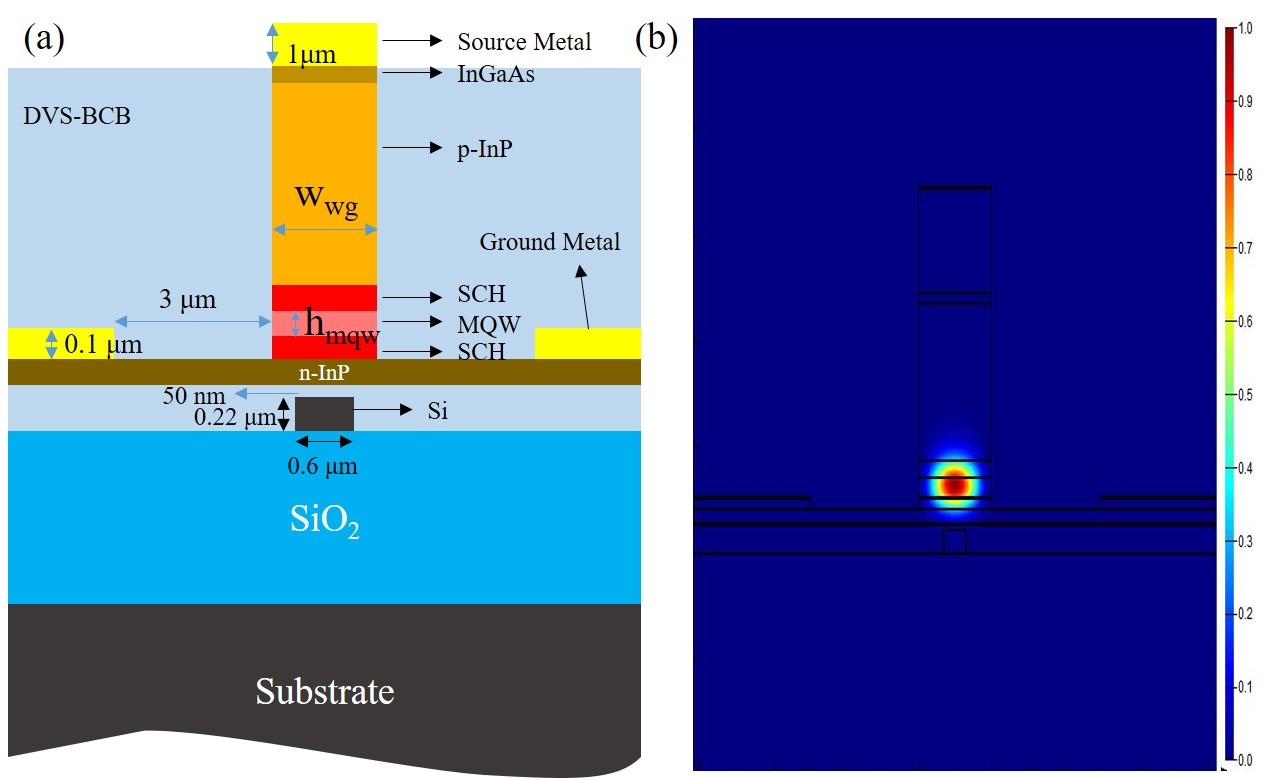
\includegraphics[width=12cm]{./Pictures/fig_ch2_rect_structure_mode.jpg}
	\caption{(a) 矩形波导截面示意图;(b) 矩形波导模场分布图,其中$w_{wg} = 2~ \mu m, h_{mqw} = 0.15 ~\mu m, \lambda_0 = 1.55\mu m$}
	\label{fig_ch2_rect_structure_mode}
\end{figure}

矩形波导的截面图如图\ref{fig_ch2_rect_structure_mode}(a)所示。其有很多参数需要设计,比如波导的宽度$w_{wg}$,多量子的厚度$h_{mqw}$,金属电极的厚度,地电极和波导之间的距离。在此,我们首先考虑波导宽度和多量子阱厚度对波导光学性能上的影响。而金属电极的厚度和地电极和波导之间的距离虽然在光学上只会影响波导损耗,但是对微波上的影响更为明显。在光学性能分析中,金属电极的设计参数如图\ref{fig_ch2_rect_structure_mode}(a)所示。图\ref{fig_ch2_rect_structure_mode}(b)展示了当$w_{wg} = 2 ~\mu m, h_{mqw} = 0.15 ~\mu m$, 工作波长$\lambda_0 = 1.55~\mu m$时的模场分布。可以看到大部分光场集中在多量子阱区域。


下面分析当矩形波导的宽度从$0.8 ~\mu m$变化到$3 \mu m$, 量子阱的高度从 $0.05 ~\mu m$变化到$0.2 ~\mu m$时,波导的等效折射率$n_{eff}$,群折射率$n_g$,损耗$loss$和光强在量子阱所占的百分比,即约束因子(confinement factor),的变化。我们采用Lumerical公司的MODE Solution进行计算\cite{modesolution},结果如图所示\ref{fig_ch2_rect_property}。

\begin{figure}[htb]
\small
\subfigure[]{
	\begin{minipage}[]{0.5\textwidth}
		\centering
		\label{fig_ch2_rect_neff}
		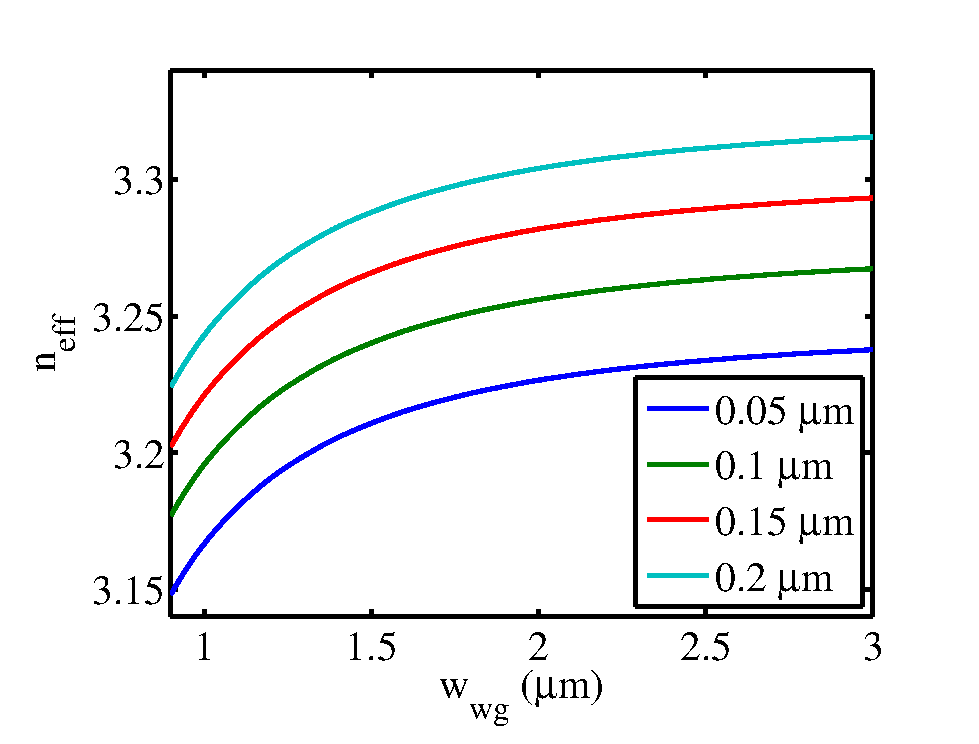
\includegraphics[width=8cm]{./Pictures/fig_ch2_rect_neff.eps}
	\end{minipage}}
\subfigure[]{
	\begin{minipage}[]{0.5\textwidth}
		\centering
		\label{fig_ch2_rect_ng} %% label for second subfigure
		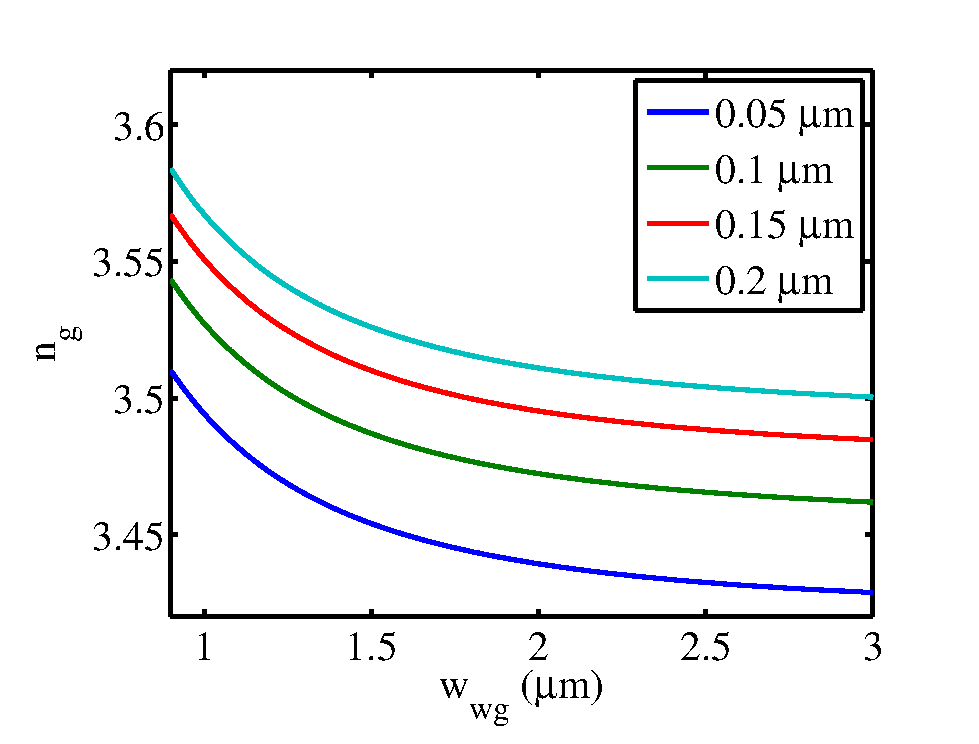
\includegraphics[width=8cm]{./Pictures/fig_ch2_rect_ng.eps}
	\end{minipage}}
\subfigure[]{
	\begin{minipage}[]{0.5\textwidth}
		\centering
		\label{fig_ch2_rect_loss} %% label for second subfigure
		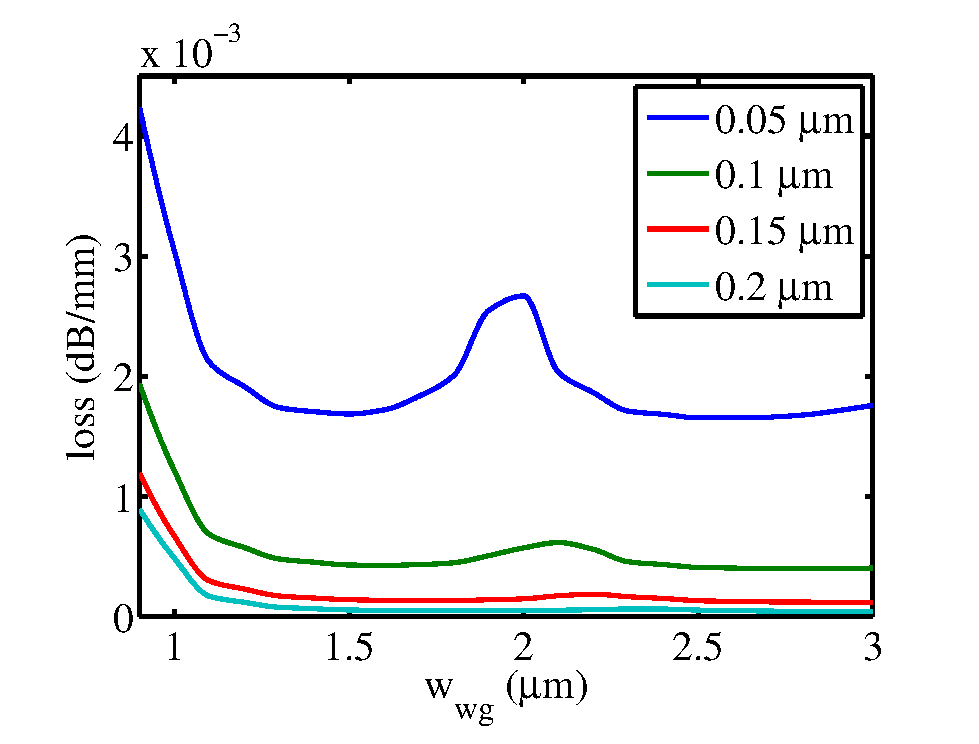
\includegraphics[width=8cm]{./Pictures/fig_ch2_rect_loss.eps}
	\end{minipage}}
\subfigure[]{
	\begin{minipage}[]{0.5\textwidth}
		\centering
		\label{fig_ch2_rect_confinement} %% label for second subfigure
		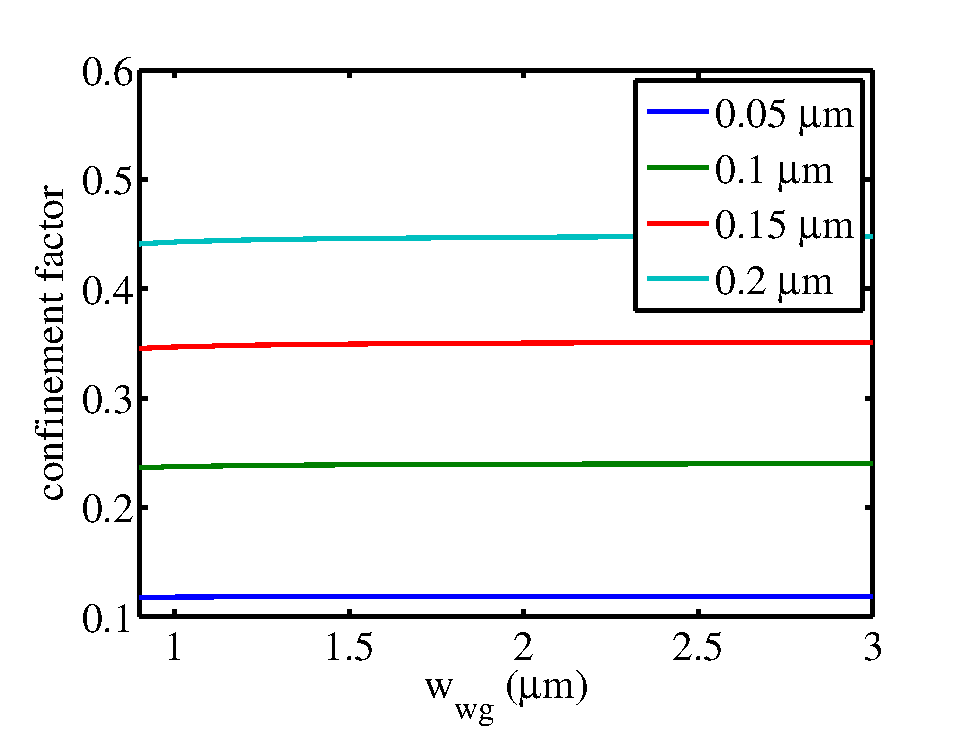
\includegraphics[width=8cm]{./Pictures/fig_ch2_rect_confinement.eps}
	\end{minipage}}
\caption{图(a)-(d)分别是在不同量子阱厚度下,矩形波导的$n_{neff}, n_g, loss, confinement~factor$随$w_{wg}$的关系,工作波长$\lambda_0 = ~1.55\mu m$}
\label{fig_ch2_rect_property}
\end{figure}

从图\ref{fig_ch2_rect_neff}可以看到,随着矩形波导的宽度和量子阱厚度的增加,等效折射率都在递增。而随着宽度的增加,等效折射率趋于稳定,但是随着高度的增加等效折射率线性增加。不过,高度继续增加的话,等效折射率也会逐渐趋向于量子阱材料的折射率。

等效折射率表征了光相位的变化速度,而调制器光信号的传输速度则与群折射率有关。从图\ref{fig_ch2_rect_ng}可以看到,随着波导宽度的增加,群折射率逐渐减小,而量子阱厚度增加群折射率反而提高。

波导的损耗可以从图\ref{fig_ch2_rect_loss}看出,随着波导宽度和量子阱高度的增加,越来越多的光约束在量子阱区域,因此损耗也会降低。可以看到当量子阱厚度大于$0.15~ \mu m$,波导宽度大于$1~ \mu m$时,损耗对波导尺寸的变化不敏感。

从图\ref{fig_ch2_rect_confinement}可以看到量子阱的厚度逐渐增加约束因子逐渐提高,约束因子对波导的宽度不敏感。当波导宽度从$1 ~\mu m$变化到$3 ~\mu m$,约束因子只有不到1\%的提高。

下面我们将分析矩形波导的微波特性。我们采用Ansys公司的HFSS进行计算\cite{ansyshfss}。图\ref{fig_ch2_rect_microwave_mode_equal_circuits}(a)展示了当$w_{wg} =~2 \mu m, h_{mqw} =~ 0.15 \mu m$,微波频率$f_m =~ 40 GHz$时的微波模场的分布。相比图\ref{fig_ch2_rect_structure_mode}(a)所示的光场分布图,微波分布图大部分能量也是集中于MQW和SCH本征层中,但是由于微波波长远大于通信波段的波长,因此微波更多的能量泄漏到量子阱外面。
\begin{figure}[htb]
	\centering
	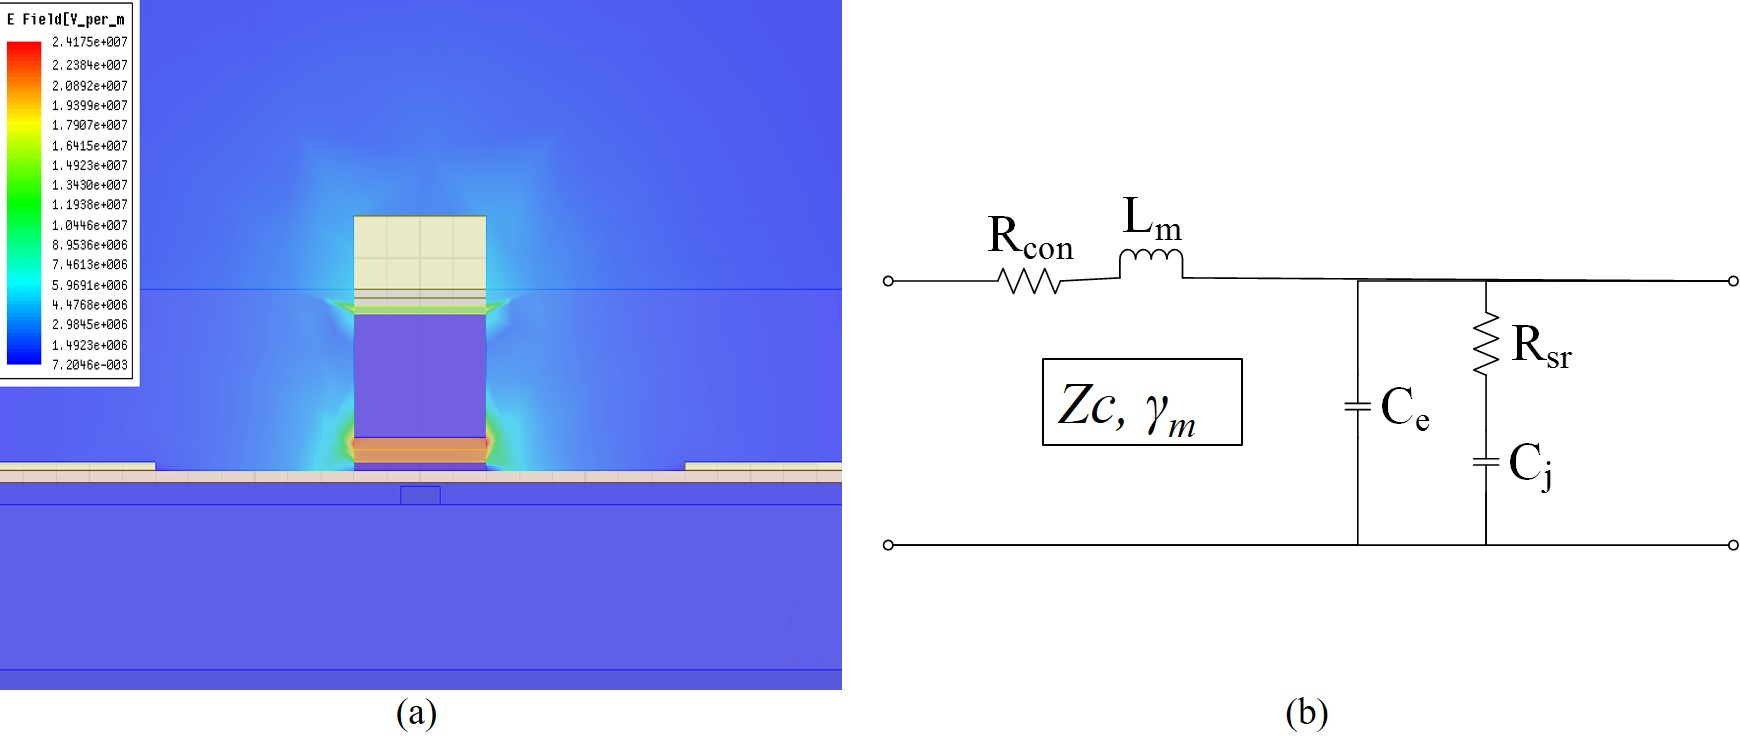
\includegraphics[width=12cm]{./Pictures/fig_ch2_rect_microwave_mode_equal_circuits.jpg}
	\caption{(a) 矩形波导微波$f_m = 40~GHz$的模式分布,其中$w_{wg} = 2~\mu m, h_{mqw} = 0.15~\mu m$;(b) 微波小信号等效电路模型}
	\label{fig_ch2_rect_microwave_mode_equal_circuits}
\end{figure}

由于矩形波导微波上对应的结构属于微带线(microstrip  line)结构,色散比较小,群折射率和等效折射率相同。描述微波的模式除了用等效折射率$n_m$外,还需要用本征阻抗(Characteristic Impedance,$Z_C$)来描述电学性能。我们可以采用微波小信号等效电路用金属电阻$R_{con}$,串联电阻$R_{sr}$,结电容$C_j$,寄生电容$C_e$,金属电感$L_m$,来表述$n_m, Z_C$。
\begin{equation}
\label{Equ:zc}
Z_C(\omega) = \sqrt{\frac{Z_S(\omega)}{Y_p(\omega)}}
\end{equation}
\begin{equation}
\label{Equ:gammam}
\gamma_m(\omega) = jn_m(\omega)\frac{\omega}{c_0} + \alpha_m(\omega) = \sqrt{Z_S(\omega)Y_p(\omega)}
\end{equation}
其中
\begin{equation}
\label{Equ:zs}
Z_S(\omega) = R_{con}+j\omega L_m
\end{equation}
\begin{equation}
\label{Equ:yp}
Y_p(\omega) = \frac{j\omega C_j}{1+j\omega C_jR_{sr}}+j\omega C_e
\end{equation}
根据文献[\citenum{li1999ultrahigh}]近似可得:
\begin{equation}
\label{Equ:zcsimple}
Z_C = \sqrt{\frac{L_m}{C_j+C_e}}
\end{equation}
\begin{equation}
\label{Equ:nmsimple}
n_m = \frac{c_0}{\omega}\left(\frac{R_{con}}{2Z_C} + \frac{\omega^2}{2}C^2_jR_{sr}Z_C\right)
\end{equation}
\begin{equation}
\label{Equ:alphasimple}
\alpha_m = \omega\sqrt{L_m(C_j+C_e)}
\end{equation}
从公式\ref{Equ:zcsimple}和\ref{Equ:alphasimple}可以看出,通过减小电容,我们能够同时增大特征阻抗和减小微波损耗。从图\ref{fig_ch2_rect_microwave_mode_equal_circuits}(a)可以看出本征层MQW和SCH是结电容器,微波的大部分能量集中于此。因此,通过增加本征层的厚度或者波导的宽度可以减小电容,提高阻抗。但是增加本征层的厚度,同时增加了所需的调制器电压。另外考虑到当量子阱的厚度小于$0.1 ~\mu m$时,光学损耗明显增加,如图\ref{fig_ch2_rect_loss}。因此我们只分析当量子阱厚度为为$0.15~ \mu m$和$0.2 ~\mu m$时的特性。
\begin{figure}[htb]
	\small
	\subfigure[]{
		\begin{minipage}[]{0.5\textwidth}
			\centering
			\label{fig_ch2_rect_zc}
			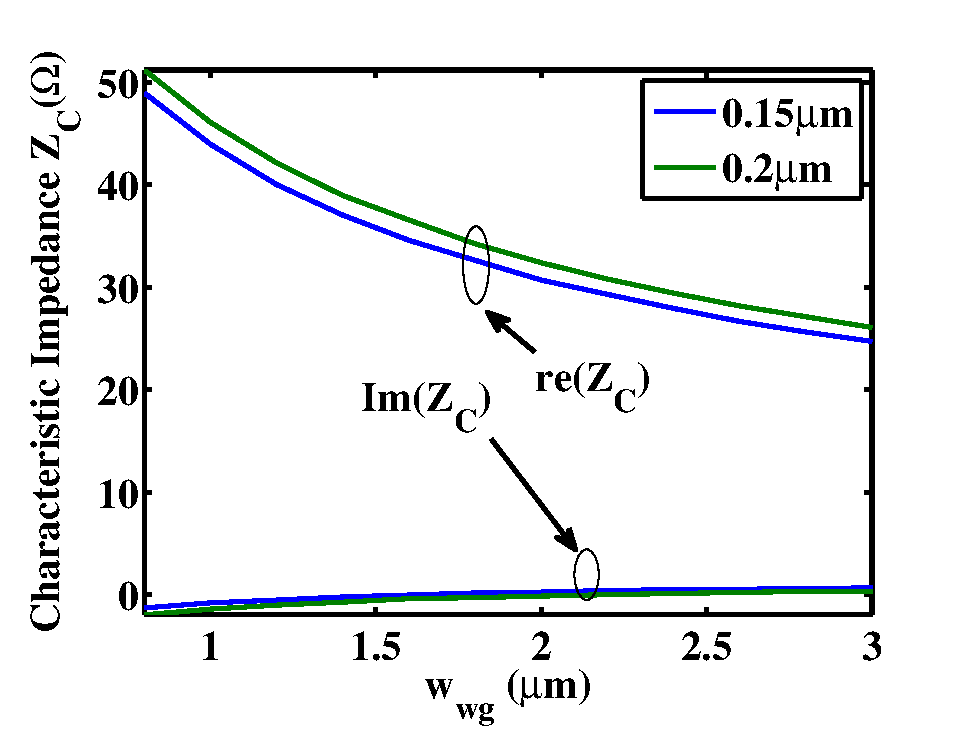
\includegraphics[width=8cm]{./Pictures/fig_ch2_rect_zc.eps}
		\end{minipage}}
	\subfigure[]{
		\begin{minipage}[]{0.5\textwidth}
			\centering
			\label{fig_ch2_rect_neff_ng} %% label for second subfigure
			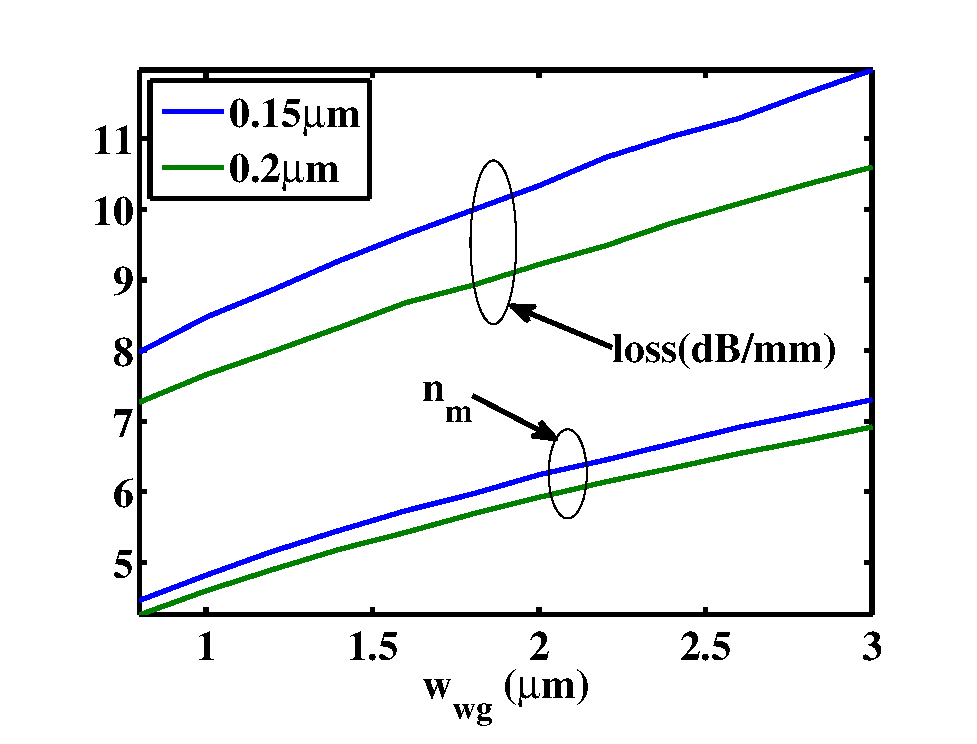
\includegraphics[width=8cm]{./Pictures/fig_ch2_rect_neff_ng.eps}
	\end{minipage}}
\caption{(a), (b)分别是$f_m = 40~GHz$时,在不同量子阱厚度下,矩形波导微波的本征阻抗$Z_C$,微波损耗$loss$,微波等效折射率$n_m$随$w_{wg}$的关系}
\label{fig_ch2_rect_microwave_property}	
\end{figure}
从图\ref{fig_ch2_rect_zc}可以看出,当波导宽度逐渐减小时或者量子阱厚度逐渐增大,导致结电容减小,因而本征阻抗逐渐提高。当$w_{wg} = 0.8~ \mu m$时,特征阻抗达到50~ $\Omega$。并且,量子阱厚度从0.15~$\mu m$增加到$0.2~\mu m$,本征阻抗变化量小。从图\ref{fig_ch2_rect_neff_ng}可以看出,微波损耗和微波的等效折射率随着同样也随着结电容的减小而减小。本征阻抗,微波损耗,微波等效折射率的变化与公式\ref{Equ:zcsimple},\ref{Equ:nmsimple},\ref{Equ:alphasimple}描述一致。

完美的行波电极调制器,需要满足微波的和光波群速度匹配,微波电阻和$50~\Omega$匹配。而目前,文献[\citenum{tang201150, zhang1999traveling}]中所展示的利用行波电极的电吸收光调制器,都没有达到这两点。之前的研究人员,通常采用分段式传输线电极,通过高阻抗高群速度和低阻抗低群速度的两种微波电极结构在小于微波波长尺寸内相互组合,达到阻抗匹配,相速度近似匹配的条件,以实现高的调制速度\cite{tang2012over,yuphd,Robertphd}。不过,分段传输线的电极结构尺寸大于行波电极结构。而在硅基混合集成平台上通过减小波导的宽度,以及合适量子阱高度,就能实现标准50~ $\Omega$完美匹配。之所以,在之前的InP基电吸收吸收光调制器中无法通过这种方式实现完美的阻抗匹配,是因为InP基的电吸收光调制器的纵向光约束能力太弱,无法实现宽度小于1~$\mu m$低损耗的波导。

借助于硅基混合集成平台能实现窄波导的特点,我们下面我们分析这种结构的调制器用行波电极的电光调制带宽。我们采用的量子阱高度是$0.187~ \mu m$与文献[\citenum{tang201150}]保持一致。当波导宽度$w_{wg} = 0.8~ \mu m$时,光学$1.55~ \mu m$的$n_g = 3.6, loss = 1.9 \times 10^{-3} ~dB/cm^{-1} $,而微波的本征阻抗$Z_C$,微波损耗$loss$,微波等效折射率$n_m$随工作频率$f$的关系如图\ref{fig_ch2_rect_freq_property}所示。
\begin{figure}[htb]
	\small
	\subfigure[]{
		\begin{minipage}[]{0.5\textwidth}
			\centering
			\label{fig_ch2_rect_freq_zc}
			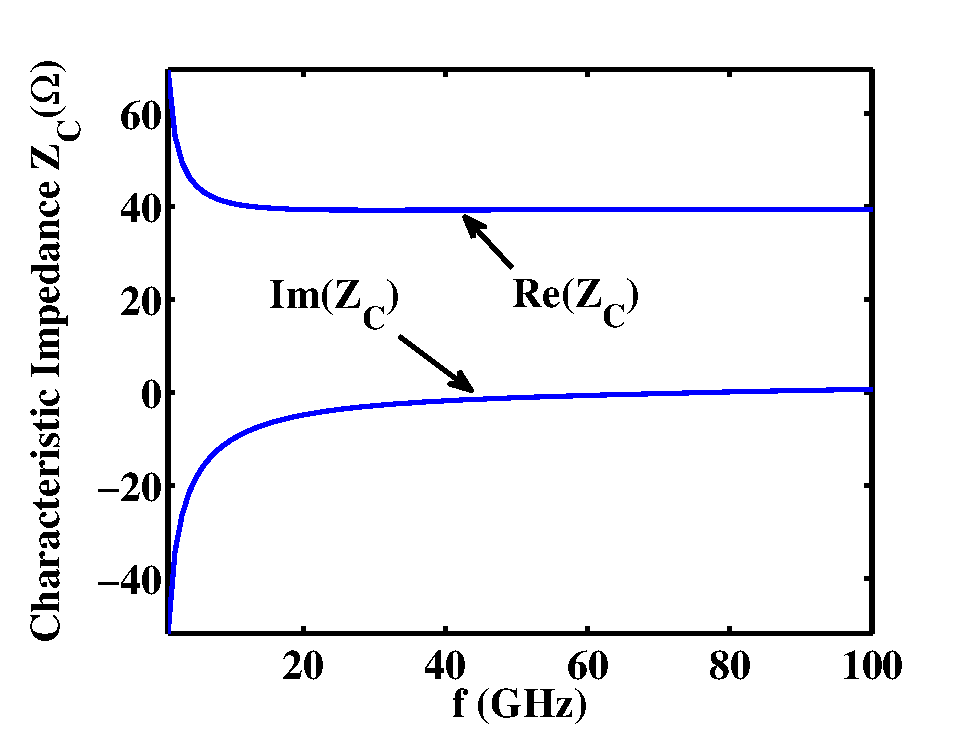
\includegraphics[width=8cm]{./Pictures/fig_ch2_rect_freq_zc.eps}
	\end{minipage}}
	\subfigure[]{
		\begin{minipage}[]{0.5\textwidth}
			\centering
			\label{fig_ch2_rect_freq_neff_loss} %% label for second subfigure
			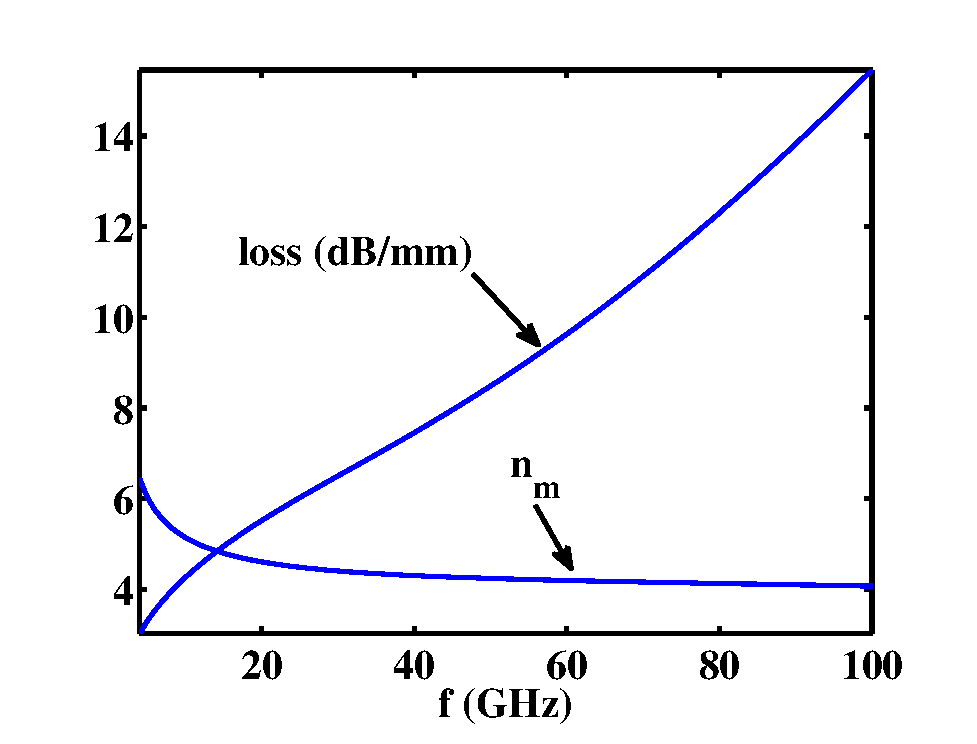
\includegraphics[width=8cm]{./Pictures/fig_ch2_rect_freq_neff_loss.eps}
		\end{minipage}}
\caption{(a), (b)分别是$w_{wg} = 0.8 ~\mu m, h_{mqw} = 0.187 ~\mu m$时,在不同量子阱厚度下,矩形波导微波的本征阻抗$Z_C$,微波损耗$loss$,微波等效折射率$n_m$随频率$f$的关系}
\label{fig_ch2_rect_freq_property}	
\end{figure}

根据波导在光学和微波的特性,计算电吸收调制器的调制带宽如下式\cite{li1999ultrahigh, tang2008design}:
\begin{equation}
\label{Equ:eoresponse}
R_{EO} = \left|\frac{1}{1+j\omega R_{rs} C_j}\frac{T}{1-\Gamma_L \Gamma_S  e^{-2 \gamma_m L} } \left\{\frac{e^{(j\beta_o-\gamma_m)L}-1}{(j\beta_o-\gamma_m)L}+\Gamma_L e^{-2\gamma_m L} \frac{e^{(j\beta_o+\gamma_m)L}-1}{(j\beta_o+\gamma_m)L} \right\} \right|^2,
\end{equation}
其中,$\beta_o = 2n_g\pi/\lambda_0, \lambda_0 = 1.55~\mu m $;微波反射系数$\Gamma_S=(Z_S-Z_C)/(Z_S+Z_C)$;$\Gamma_L=(Z_L-Z_C)/(Z_L+Z_C)$,$Z_S, Z_L$是源和负载的特征阻抗,在此我们取标准的$50~ \Omega$;调制器长度$L = 100~ \mu m$;依据文献[\citenum{tang2012over}],我们取$R_{rs} C_j=1.3~ ps$。图\ref{fig_ch2_rect_3dB_S11}展示了电光响应$R_{EO}$的带宽和微波的反射系数$S_{11}$的幅值。从图\ref{fig_ch2_rect_3dB}可以看到$R_{EO}$的3~dB带宽$f_{3dB}\approx ~100 GHz$,并且图\ref{fig_ch2_rect_S11}展示了微波的反射系数在0~GHz到100~GHz的范围内都低于-25~dB。而目前最好的硅基混合集成光调制器,利用分段传输线式电极,其3~dB带宽达到74~GHz,反射系数在高频也无法保持在-20~dB以下\cite{tang2012over}。
\begin{figure}[htb]
	\small
	\subfigure[]{
		\begin{minipage}[]{0.5\textwidth}
			\centering
			\label{fig_ch2_rect_3dB}
			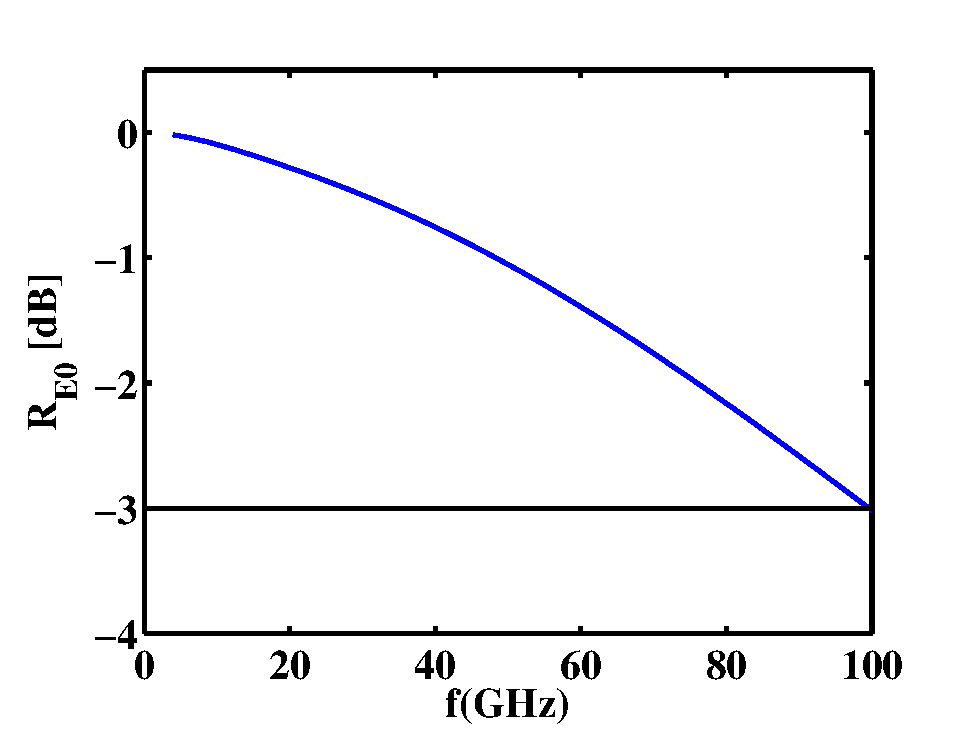
\includegraphics[width=8cm]{./Pictures/fig_ch2_rect_3dB.eps}
		\end{minipage}}
	\subfigure[]{
		\begin{minipage}[]{0.5\textwidth}
			\centering
			\label{fig_ch2_rect_S11} %% label for second subfigure
			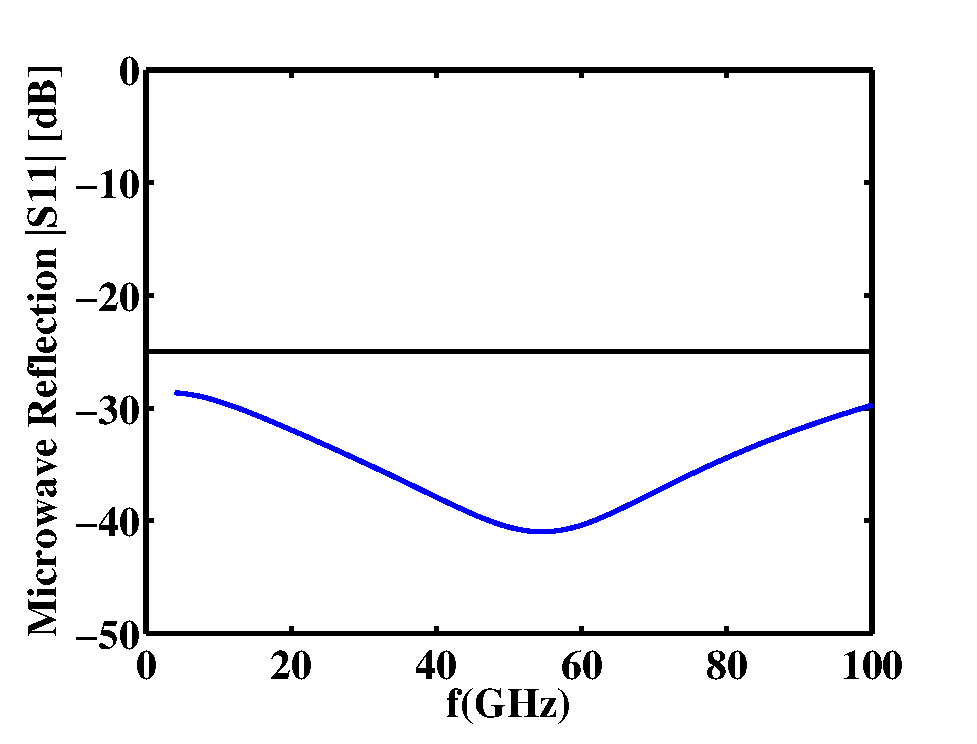
\includegraphics[width=8cm]{./Pictures/fig_ch2_rect_S11.eps}
		\end{minipage}}
\caption{(a)矩形波导调制器的电光调制器带宽$R_{EO}$;(b)矩形波导调制器的微波反射系数$|S_{11}|$}
\label{fig_ch2_rect_3dB_S11}	
\end{figure}
		
\subsection{蘑菇型波导的设计}
蘑菇型波导是利用MQW和SCH材料与InP有选择性腐蚀的特点,实现MQW和SCH区域的宽度小于p-InP层的宽度,从而降低波导的结电容$C_j$。蘑菇型波导可以先定义宽的波导掩膜,或者直接用比较宽的p-InP作为掩膜,再利用选择性腐蚀液,将量子阱区域内掏(undercut)变窄,从而降低了光刻精度,可用接触式光刻制作,因此被广泛用于电吸收光调制器\cite{chiu2005enhanced, kuo2008high, tang201150, tang2012over, tang2012energy, chen2011forty}。

蘑菇型波导的截面图如图\ref{fig_ch2_ms_structure_mode}(a)所示。相比矩形波导,蘑菇型波导的宽度有更多的待定参数,在此我们限定p-InP的宽度为2.5$\mu m$,这个尺寸是可以用接触式光刻达到。而蘑菇型波导的宽度$w_{wg}$,我们定义为多量子阱区域的宽度。其他的结构参数的定义和矩形波导保持一制,见图\ref{fig_ch2_ms_structure_mode}(a)。我们首先考虑$w_{wg}$和$h_{mqw}$对波导光学性能上的影响。图\ref{fig_ch2_ms_structure_mode}(b)展示了当$w_{wg} = 2 ~\mu m, h_{mqw} = 0.15 ~\mu m$, 工作波长$\lambda_0 = 1.55~\mu m$时的模场分布。可以看到大部分光场集中在多量子阱区域。不过相比矩形波导的模式\ref{fig_ch2_rect_structure_mode}(b),蘑菇型波导中有部分光约束在硅波导中。
\begin{figure}[htb]
	\centering
	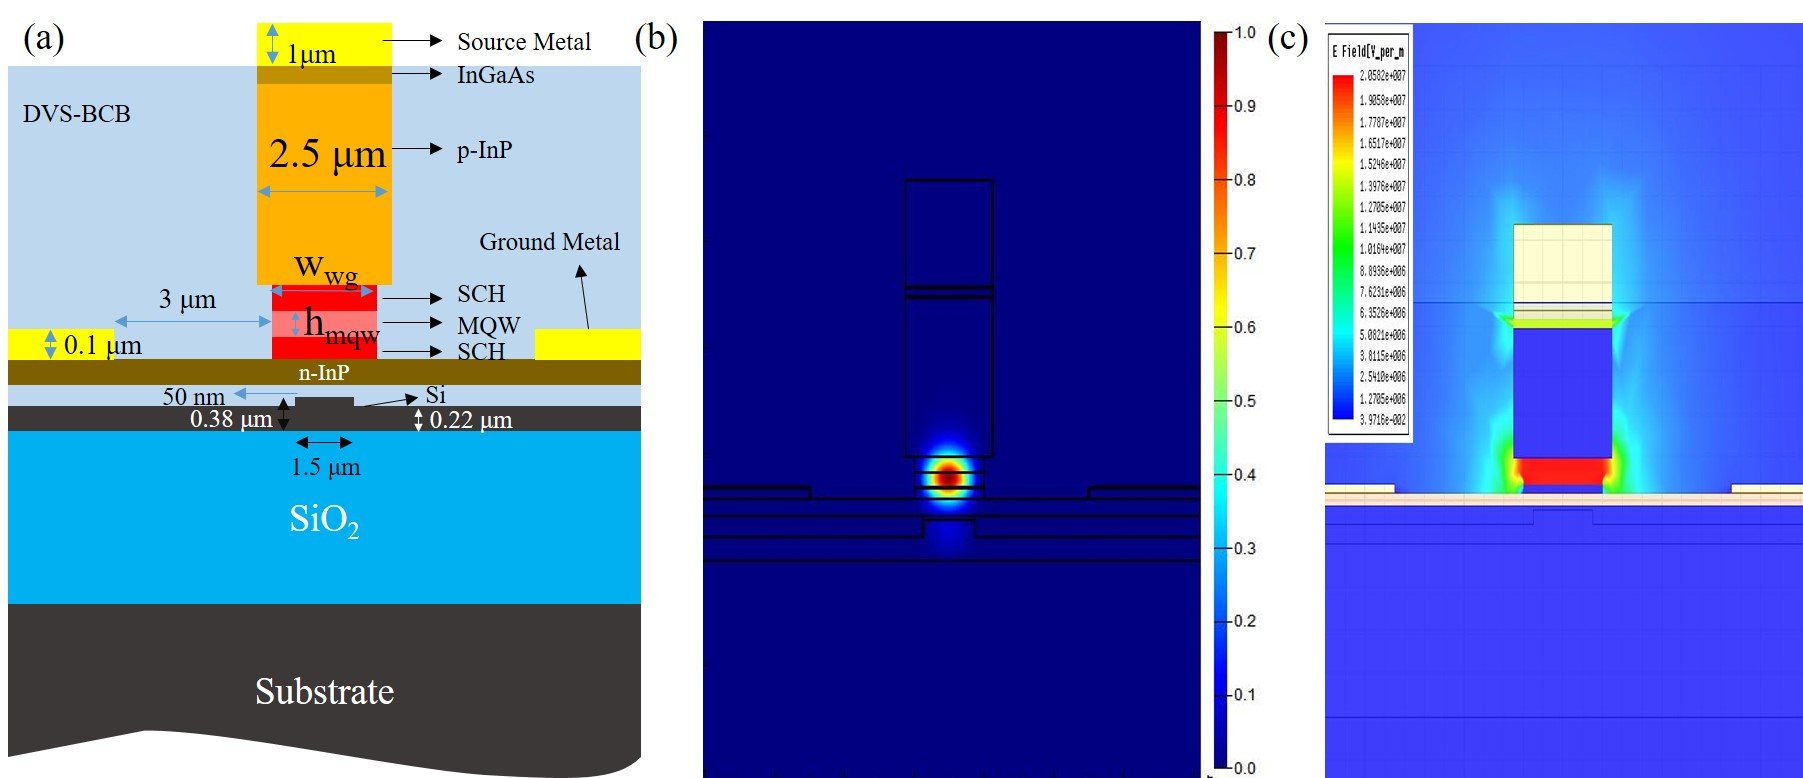
\includegraphics[width=16cm]{./Pictures/fig_ch2_ms_structure_mode.jpg}
	\caption{(a) 蘑菇型波导截面示意图;(b) 蘑菇型波导模场分布图,其中$w_{wg} = 2~ \mu m, h_{mqw} = 0.15 ~\mu m, \lambda_0 = 1.55~\mu m$;(c) 蘑菇型波导微波$f_m = 40~GHz$的模式分布,其中$w_{wg} = 2~\mu m, h_{mqw} = 0.15~\mu m$}
	\label{fig_ch2_ms_structure_mode}
\end{figure}

下面分析当蘑菇型波导的宽度从$0.8 ~\mu m$变化到$3 \mu m$, 量子阱的高度从 $0.05 ~\mu m$变化到$0.2 ~\mu m$时,蘑菇型波导的等效折射率$n_{eff}$,群折射率$n_g$,损耗$loss$和光强在量子阱所占的百分比,即约束因子(confinement factor),的变化。我们采用Lumerical公司的MODE Solution进行计算\cite{modesolution},结果如图所示\ref{fig_ch2_ms_property}。

\begin{figure}[htb]
	\small
	\subfigure[]{
		\begin{minipage}[]{0.5\textwidth}
			\centering
			\label{fig_ch2_ms_neff}
			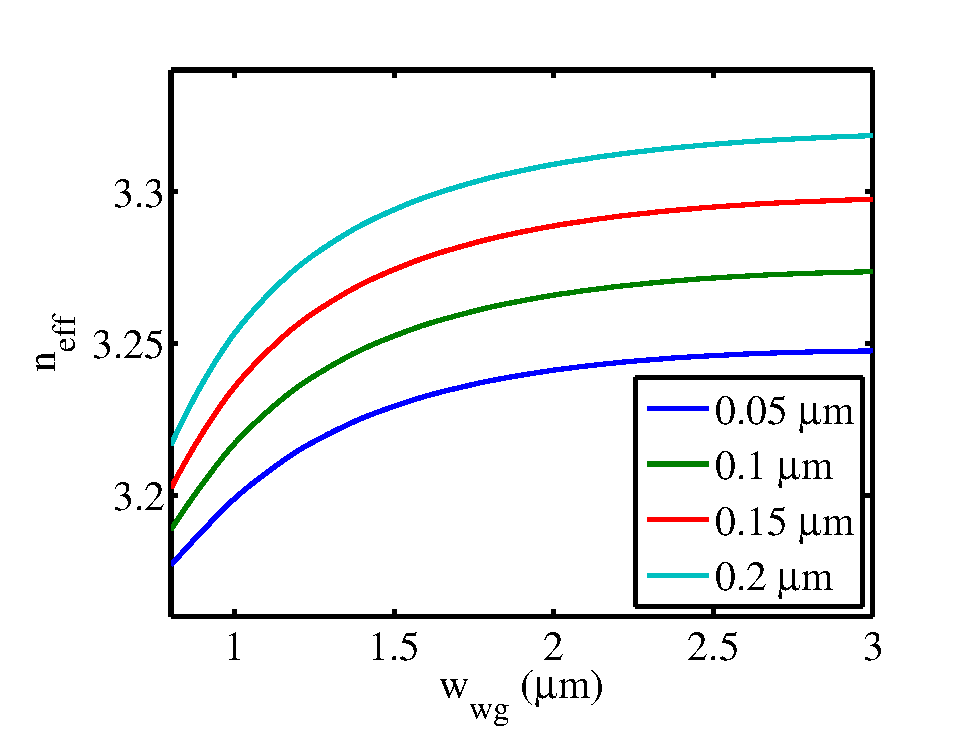
\includegraphics[width=8cm]{./Pictures/fig_ch2_ms_neff.eps}
		\end{minipage}}
	\subfigure[]{
		\begin{minipage}[]{0.5\textwidth}
			\centering
			\label{fig_ch2_ms_ng} %% label for second subfigure
			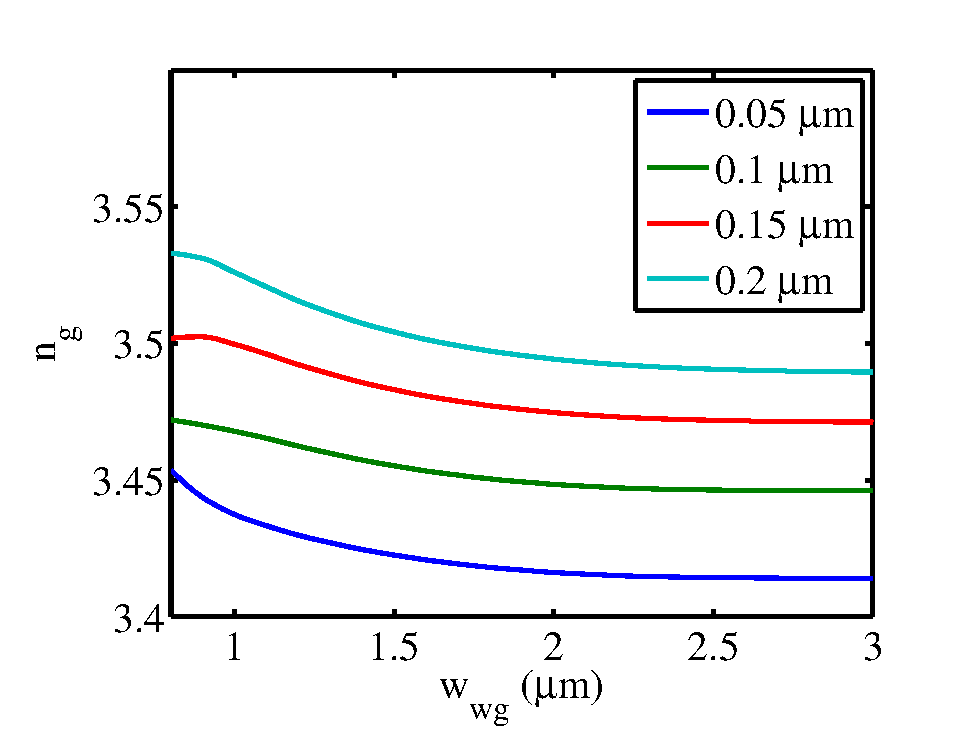
\includegraphics[width=8cm]{./Pictures/fig_ch2_ms_ng.eps}
		\end{minipage}}
	\subfigure[]{
		\begin{minipage}[]{0.5\textwidth}
			\centering
			\label{fig_ch2_ms_loss} %% label for second subfigure
			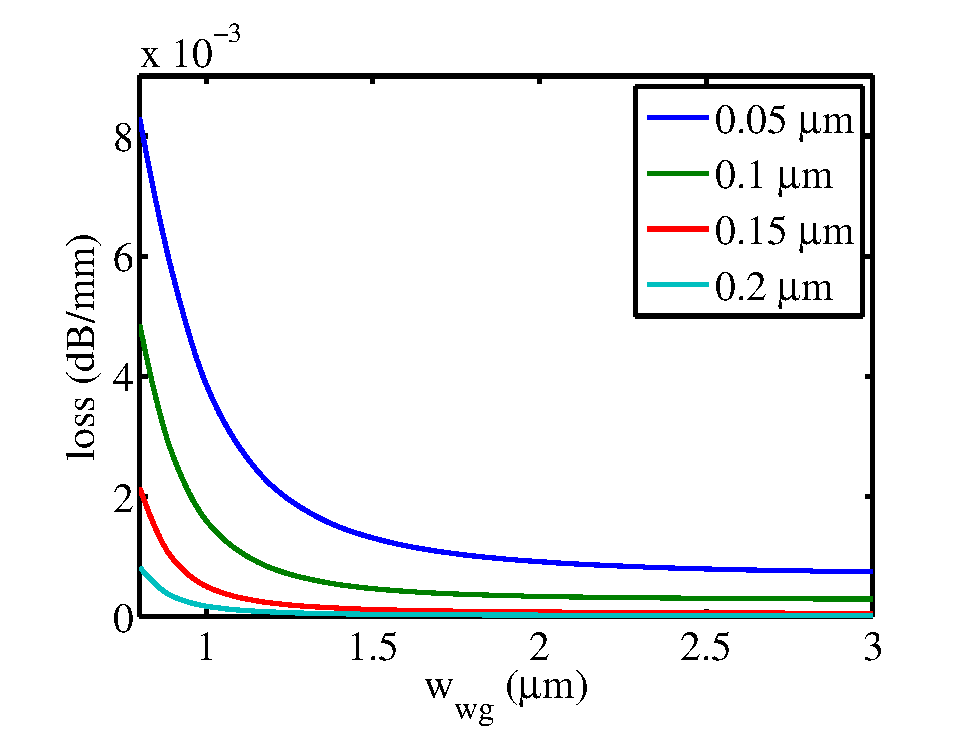
\includegraphics[width=8cm]{./Pictures/fig_ch2_ms_loss.eps}
		\end{minipage}}
	\subfigure[]{
		\begin{minipage}[]{0.5\textwidth}
			\centering
			\label{fig_ch2_ms_confinement} %% label for second subfigure
			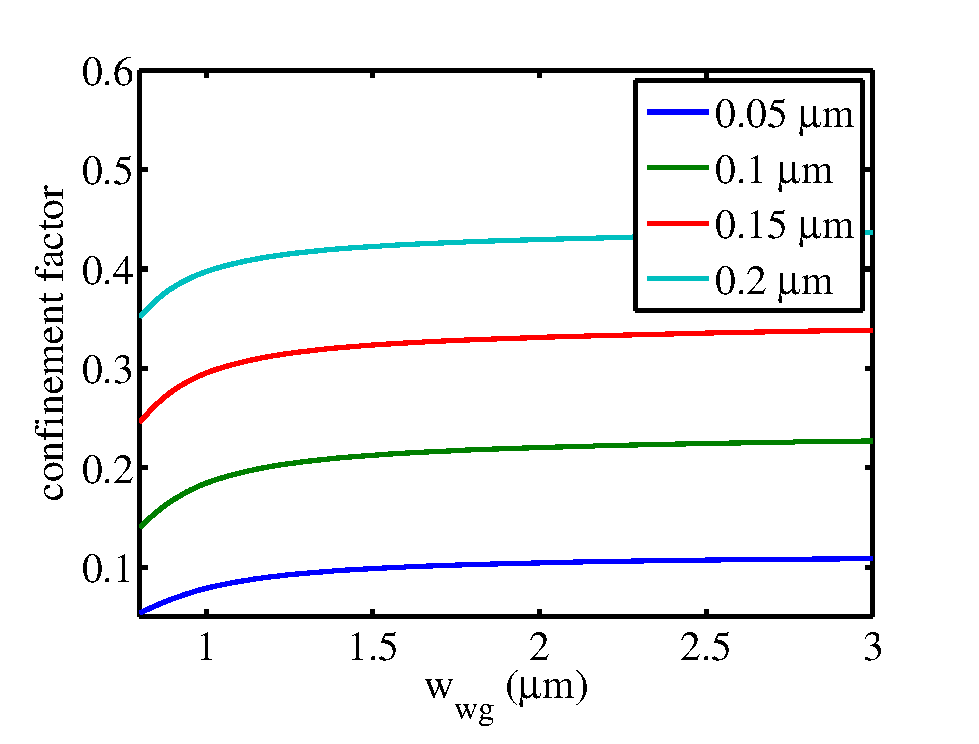
\includegraphics[width=8cm]{./Pictures/fig_ch2_ms_confinement.eps}
		\end{minipage}}
\caption{(a)-(d)分别是在不同量子阱厚度下,蘑菇型波导的$n_{neff}, n_g, loss, confinement~factor$随$w_{wg}$的关系,工作波长$\lambda_0 = ~1.55\mu m$}
\label{fig_ch2_ms_property}
\end{figure}


从图\ref{fig_ch2_ms_property}可以看到,蘑菇型等效折射率,群折射率,波导损耗,约束因子的变化趋势与矩形波导变化趋势相同。在同样的波导宽度和量子阱厚度下,蘑菇型波导的等效折射率偏大,群折射率偏小,损耗偏大,光约束能力偏小。这是由于矩形波导对光约束的更好,群折射率越大。另外蘑菇型波导相对比较宽的p-InP层,会让更多的光被上电极吸收,导致损耗偏大,光约束能力降低。

下面我们将分析蘑菇型波导的微波特性。图\ref{fig_ch2_ms_structure_mode}(c)展示了当$w_{wg} =~2 \mu m, h_{mqw} =~ 0.15 \mu m$,微波频率$f_m =40~ GHz$时的微波模场的分布,与矩形波导的微博模场分布图\ref{fig_ch2_rect_microwave_mode_equal_circuits}(a)相似,微波的大部分能量集中于MQW和SCH本征层中,部分能量集中在p-contact层。

与矩形波导分析思路相同,下面我们分析当量子阱厚度为为$0.15~ \mu m$和$0.2 ~\mu m$时蘑菇型波导的微波特性。从图\ref{fig_ch2_ms_zc}和图\ref{fig_ch2_ms_neff_ng}可以看出,当波导宽度逐渐减小或者量子阱厚度逐渐增大,蘑菇型波导的本征阻抗,微波损耗和微波等效折射率的变化趋势与矩形波导的微波特性变化趋势相同。不过,在相同波导尺寸下,这种蘑菇型波导的本征阻抗偏小,微波等效折射率偏偏大。因此,蘑菇型波导更不容易实现阻抗匹配以及微波与光波的速度匹配。
接下来,我们比较在与矩形相同波导宽度和量子阱高度下,蘑菇型波导的电光调制器带宽。当量子阱高度是$0.187~ \mu m$,波导宽度$w_{wg} = 0.8~ \mu m$工作波长为$1.55~ \mu m$时,$n_g = 3.525, loss =  2\times 10^{-3} ~dB/cm^{-1} $。此时微波的本征阻抗$Z_C$,微波损耗$loss$,微波等效折射率$n_m$随工作频率$f$的关系如图\ref{fig_ch2_ms_freq_zc}和图\ref{fig_ch2_ms_freq_neff_loss}所示。
图\ref{fig_ch2_ms_3dB}和图\ref{fig_ch2_ms_S11}分别展示了蘑菇型波导的电光响应$R_{EO}$的带宽和微波的反射系数$S_{11}$的幅值。从图\ref{fig_ch2_ms_3dB}可以看到$R_{EO}$的3~dB带宽$f_{3dB}\approx ~90 GHz$,小于矩形波导的$f_{3dB}$。并且蘑菇型波导的反射系数在25~GHz的以上时高于-25~dB,也差于矩形波导。\cite{tang2012over}。

\begin{figure}[htb]
	\small
	\subfigure[]{
		\begin{minipage}[]{0.5\textwidth}
			\centering
			\label{fig_ch2_ms_zc}
			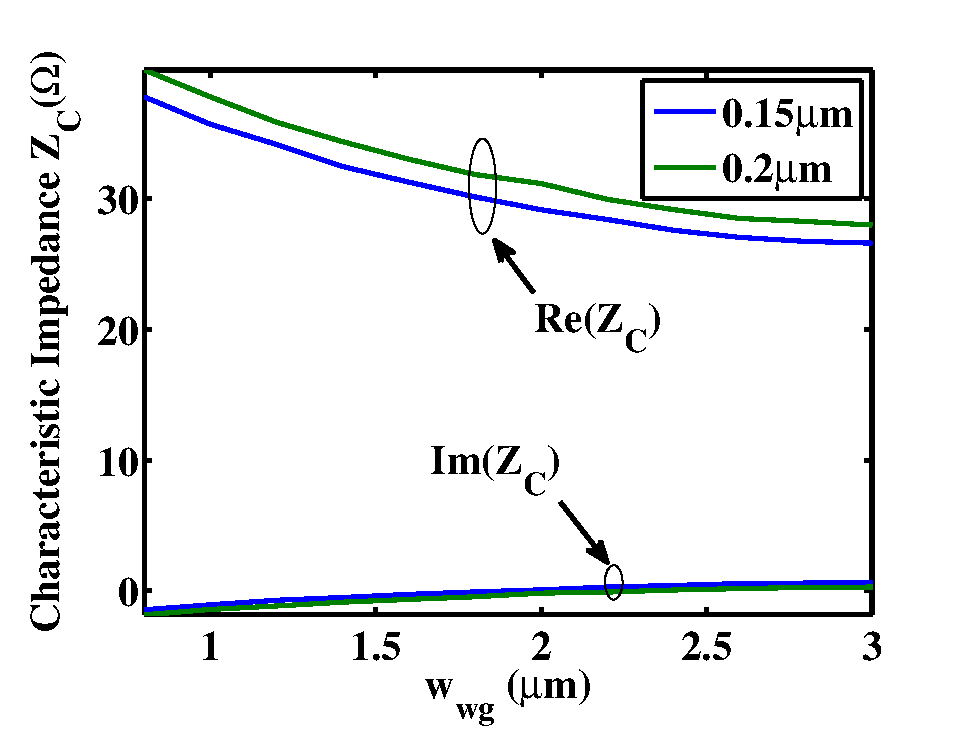
\includegraphics[width=8cm]{./Pictures/fig_ch2_ms_zc.eps}
		\end{minipage}}
		\subfigure[]{
		\begin{minipage}[]{0.5\textwidth}
			\centering
			\label{fig_ch2_ms_neff_ng} %% label for second subfigure
			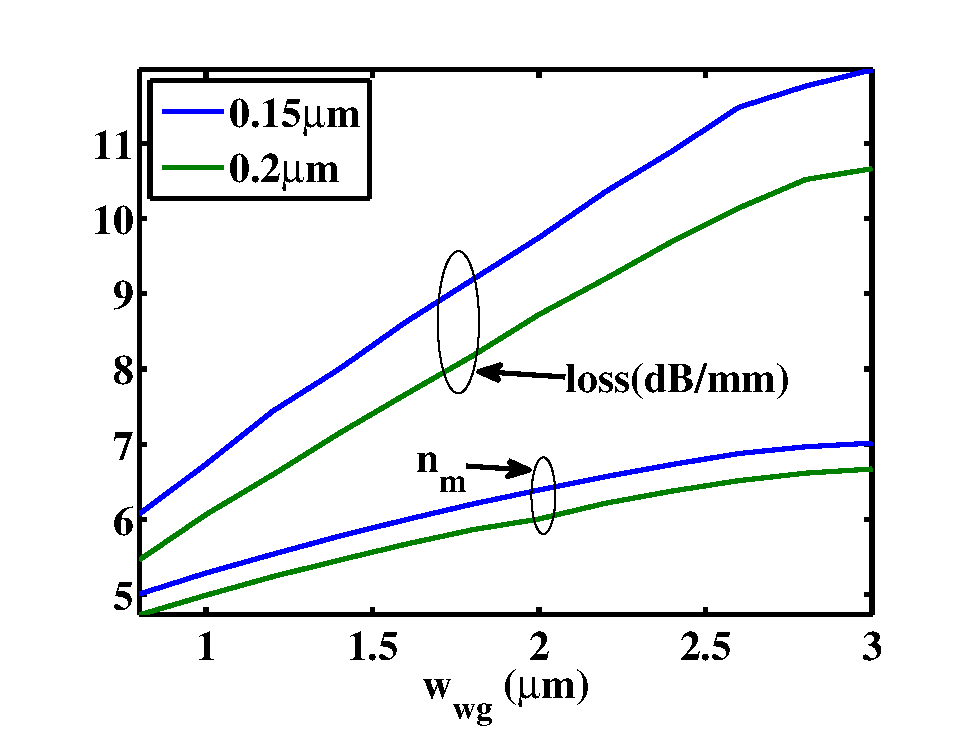
\includegraphics[width=8cm]{./Pictures/fig_ch2_ms_neff_ng.eps}
		\end{minipage}}
	\subfigure[]{
		\begin{minipage}[]{0.5\textwidth}
			\centering
			\label{fig_ch2_ms_freq_zc}
			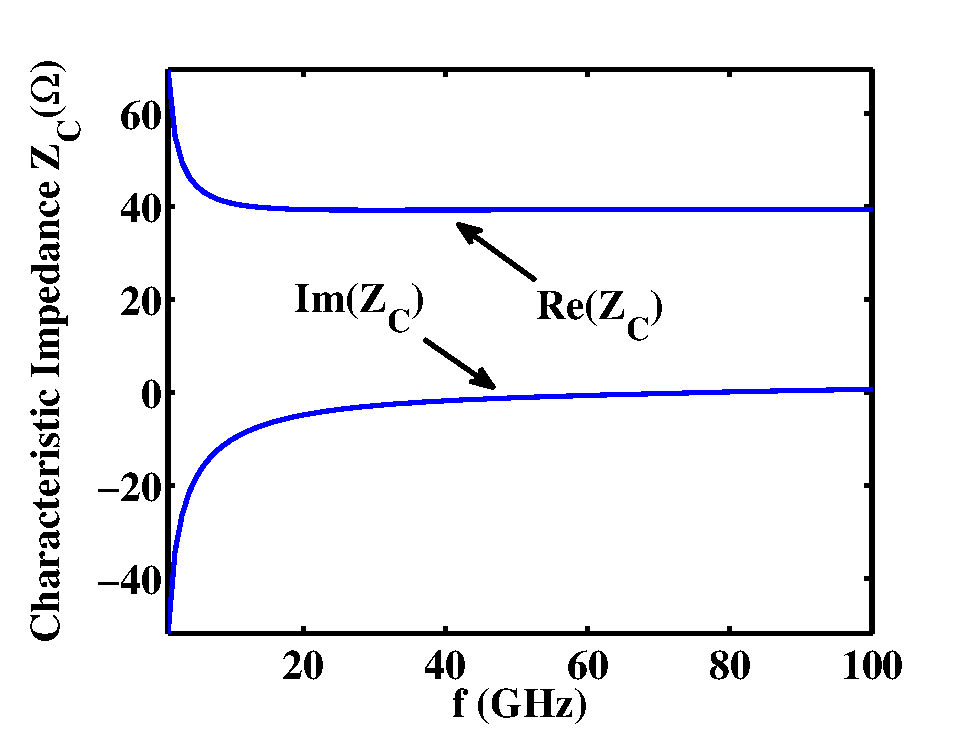
\includegraphics[width=8cm]{./Pictures/fig_ch2_ms_freq_zc.eps}
		\end{minipage}}
	\subfigure[]{
		\begin{minipage}[]{0.5\textwidth}
			\centering
			\label{fig_ch2_ms_freq_neff_loss} %% label for second subfigure
			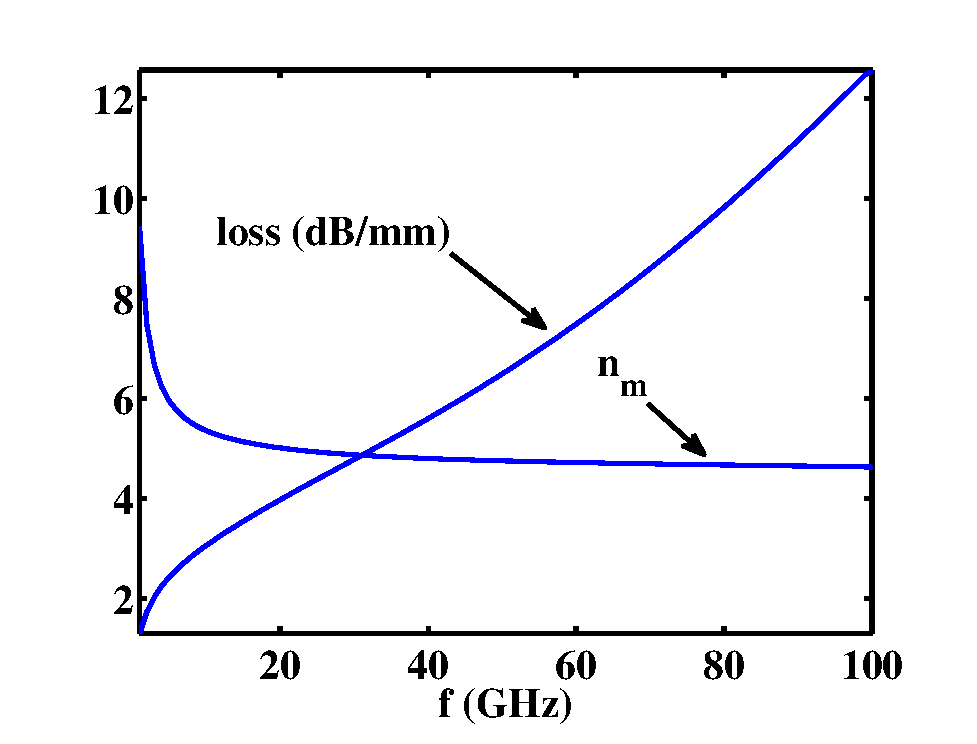
\includegraphics[width=8cm]{./Pictures/fig_ch2_ms_freq_neff_loss.eps}
		\end{minipage}}
	\subfigure[]{
		\begin{minipage}[]{0.5\textwidth}
			\centering
			\label{fig_ch2_ms_3dB} %% label for second subfigure
			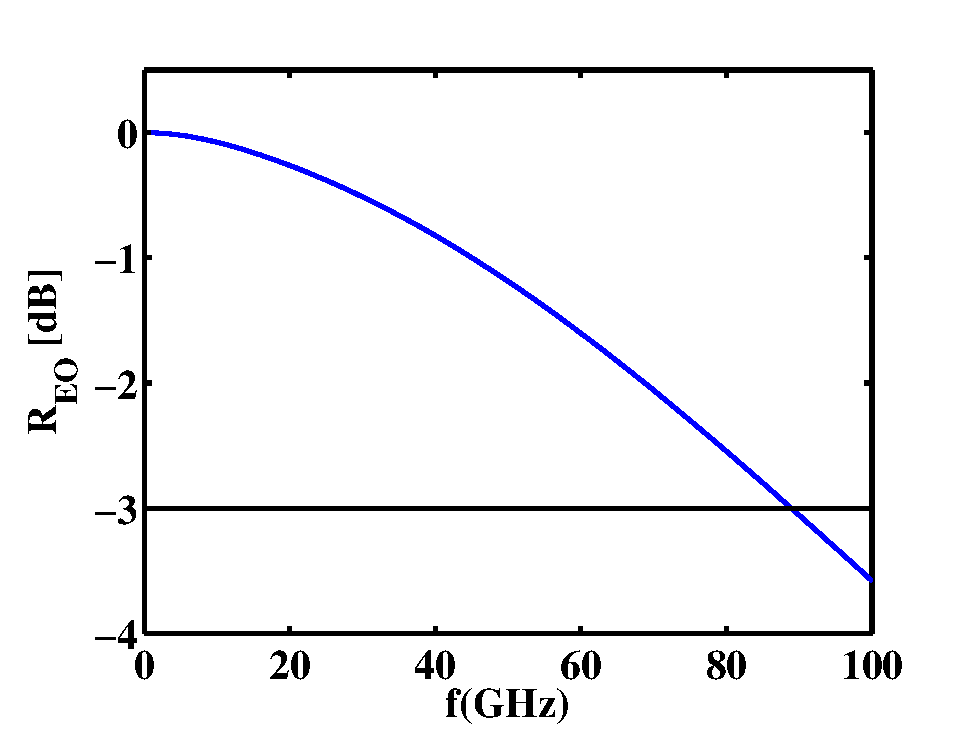
\includegraphics[width=8cm]{./Pictures/fig_ch2_ms_3dB.eps}
		\end{minipage}}
	\subfigure[]{
		\begin{minipage}[]{0.5\textwidth}
			\centering
			\label{fig_ch2_ms_S11} %% label for second subfigure
			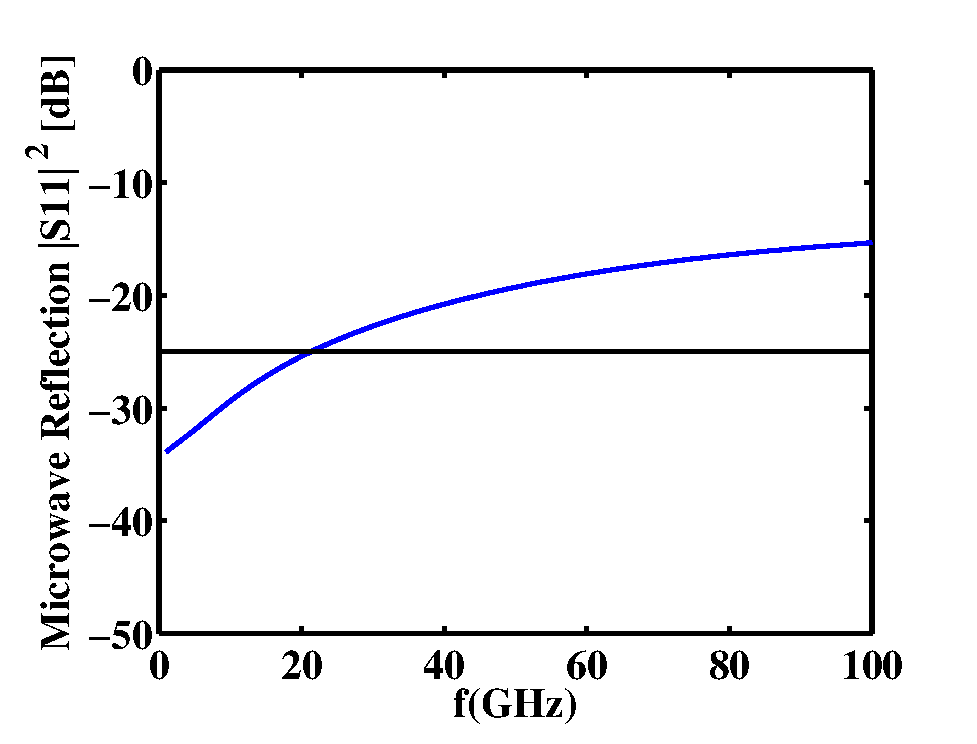
\includegraphics[width=8cm]{./Pictures/fig_ch2_ms_S11.eps}
		\end{minipage}}
	\caption{(a), (b)分别是$f_m = 40~GHz$时,在不同量子阱厚度下,蘑菇型波导微波的本征阻抗$Z_C$,微波损耗$loss$,微波等效折射率$n_m$随$w_{wg}$的关系;(c), (d)分别是$w_{wg} = 0.8 ~\mu m, h_{mqw} = 0.187 ~\mu m$时,在不同量子阱厚度下,蘑菇型波导微波的本征阻抗$Z_C$,微波损耗$loss$,微波等效折射率$n_m$随微波频率$f$的关系;(e)蘑菇型波导调制器的电光调制器带宽$R_{EO}$;(f)蘑菇型波导调制器的微波反射系数$|S_{11}|$}
	\label{fig_ch2_ms_3dB_S11}
\end{figure}

虽然远离量子阱区域的电极尺寸的变化对光波的影响十分微弱,但是,由于微波波长尺寸大,电极尺寸的变化对微波的特性影响十分明显。在此,我们分析地电极和源电极的尺寸变化对波导微波性能的影响。通过表\ref{rect_metal_influence}的分析,我们可以通过微调电极的尺寸,在不影响光波损耗的前提下,调节电极尺寸改善波导的微波特性。	
{
	\begin{table}[htb]
		\zihao{5}
		\caption{矩形或者蘑菇型波导结构,当源电极的厚度,高度,地电极的厚度和两者之间的距离变大时,微波的本征阻抗,损耗和等效折射率的变化}
		\label{rect_metal_influence}
		\centering
		\begin{tabular}[t]{lllll}
			\hline
			参数类型 &源电极的厚度 & 源电极的宽度 & 地电极的厚度& 地电极之间的距离 \\
			\hline
			本征阻抗 &   减小 & 减小 & 减小 &增大\\
			损耗  &   减小 & 减小 & 增大 &增大\\
			等效折射率 &  减小 & 减小 & 减小 &增大\\
			\hline
		\end{tabular}
	\end{table}
}

			
\section{本章小结}
在本章中,我们详细介绍了设计硅基混合集成III-V波导的两个方面。第一方米我们首先详细介绍III-V外延片量子阱结构的吸收谱计算的四个步骤。然后对于设计量子阱,这种多参数优化问题,我们首次引入了利用退火算法设计、优化量子阱结构的思路。通过合理设计退火算法中参数的取值范围,以及退火算法的权值函数,我们可以快速设计出偏振不敏感的电吸收光调制器的量子阱结构。最后,我们总结了III-V外延片的总体设计。第二方面是混合集成III-V波导尺寸尺寸的设计,我们分析了两种类型的波导,矩形波导和蘑菇型波导分析了波导宽度和多量子阱高度对波导光学和微波特性的影响,并且分析了相同尺寸下,两种结构的电光调制带宽。我们发现在相同尺寸下矩形波导可以实现阻抗匹配,而蘑菇型波导本征阻抗偏小,这导致了矩形波导可以实现$f_{3dB} = 100~GHz$的调制带宽。